\documentclass{beamer}
\usepackage[utf8]{inputenc}
\usepackage{amsmath}
\usepackage{graphicx}

\title{Colisões elásticas com Arduino}
\author{Geovanni Fernandes Garcia & N° USP: 11298560\\
        Isaias Nascimento Caetano Pinto & N° USP:  10787056}
\date{}

\begin{document}

\maketitle 

\section{Introduction}

\begin{frame}{Objetivo}
    
    \begin{itemize}
        \item Facilitar a tomada de dados para o experimento de colisão elástica
        \item Melhorar a precisão dos dados tomados
        \item Comparar a precisão dos sensores
        \item Estudar a conservação do momento linear
    \end{itemize}
    
\end{frame}

\begin{frame}{Materiais utilizados}

    Para o experimento foram utilizados:
    
    \begin{itemize}
        \item Trilho de ar
        \item Carrinhos de metal para o trilho de ar
        \item Placa de arduíno Uno
        \item Sensor de ultrassom
        \item Sensor Lidar (Infravermelho)
        \item Protoboard
        \item Suporte para o detector
        \item Balança
        \item 2 elásticos
        \item 1 cartão
    \end{itemize}
    
\end{frame}

\begin{frame}{Arranjo experimental}

    \begin{figure}
  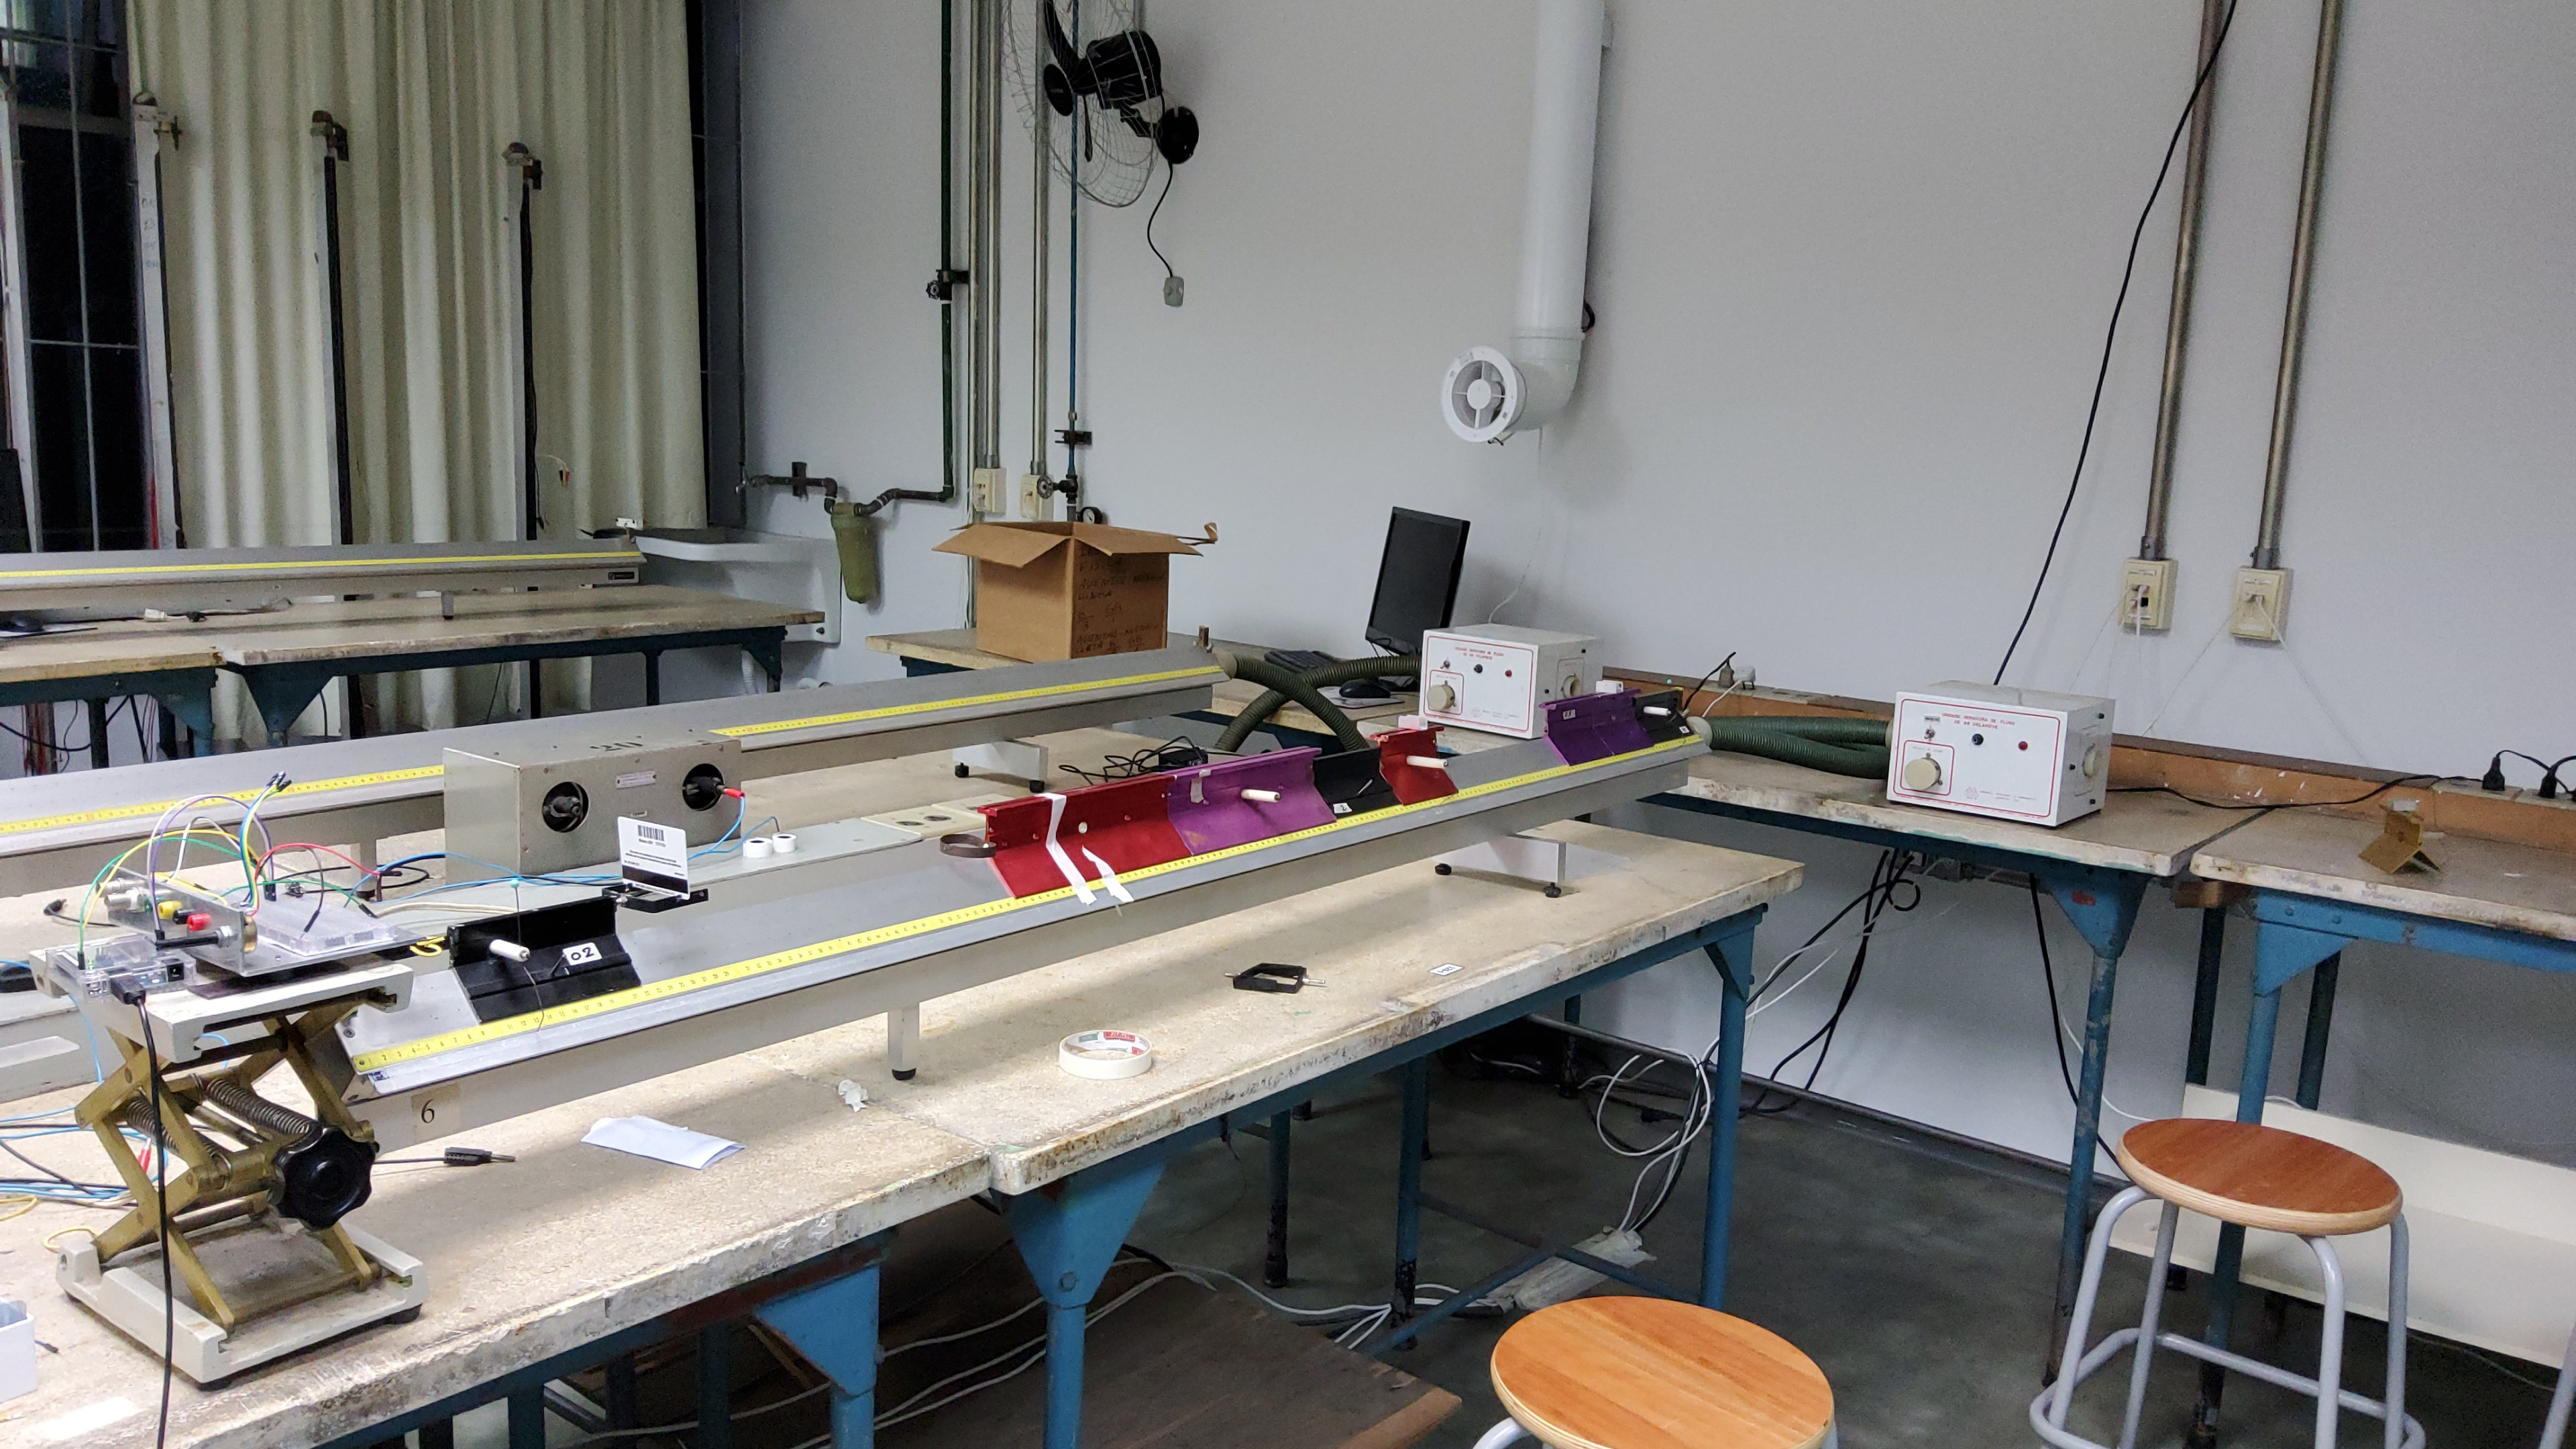
\includegraphics[width=300px]{IMG-20221206-WA0027}
  
\end{figure}

    
\end{frame}

\begin{frame}{Arranjo experimental}

    \begin{figure}
  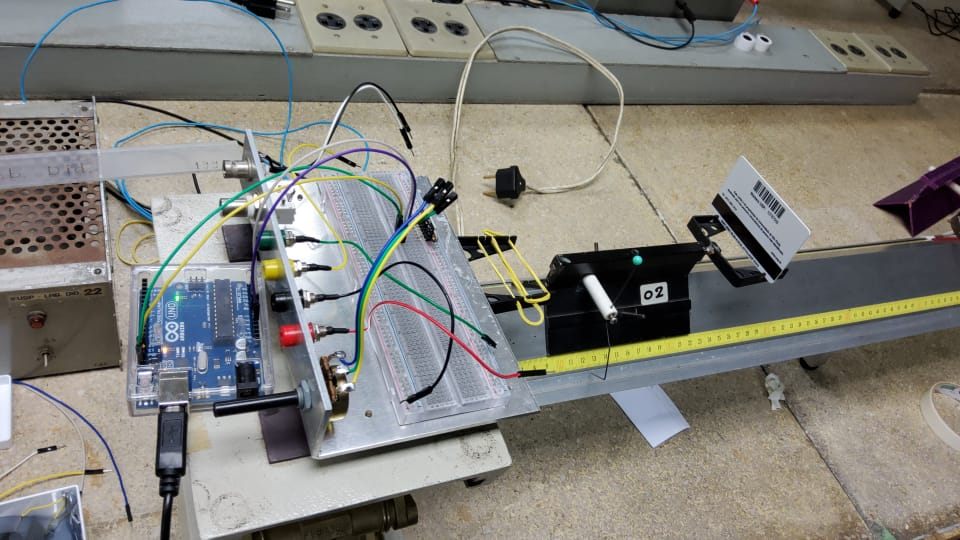
\includegraphics[width=\linewidth]{06810750-c706-4d4c-a97f-17cbf277e8f1.jpg}
\end{figure}

\end{frame}

\begin{frame}{Arranjo experimental}
    \begin{figure}
  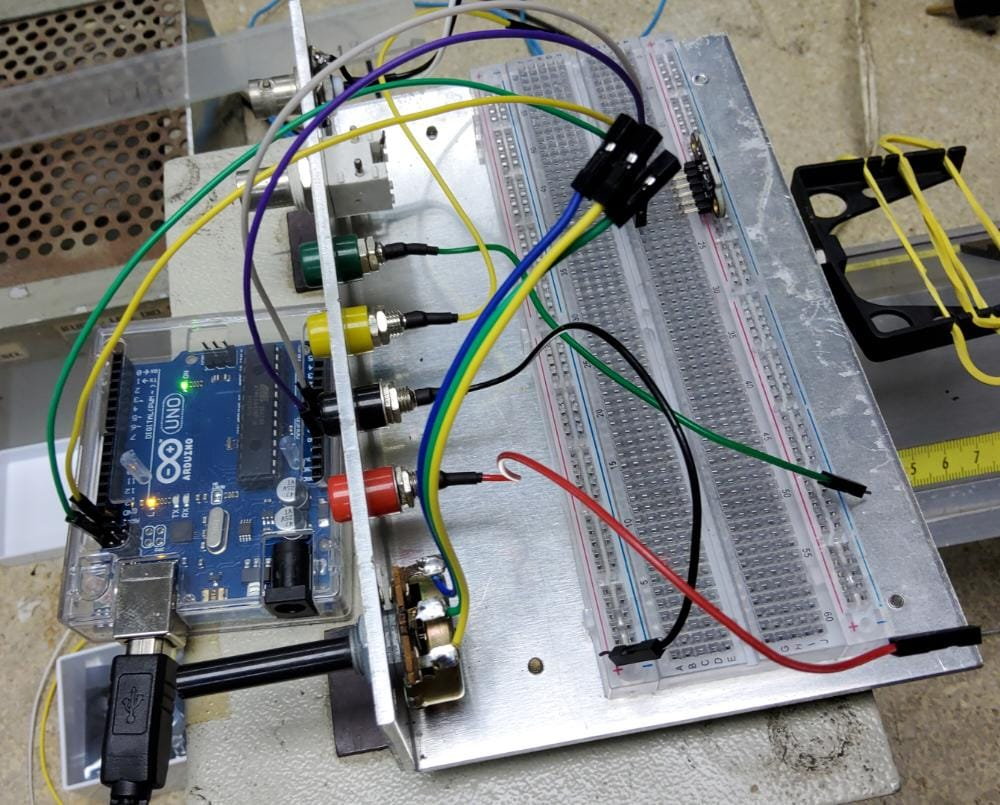
\includegraphics[width=220px]{86cf2d62-b209-48d7-8f31-87e7bdd2bca0.jpg}
\end{figure}
    
\end{frame}

\begin{frame}{Arranjo experimental}

    \begin{figure}
  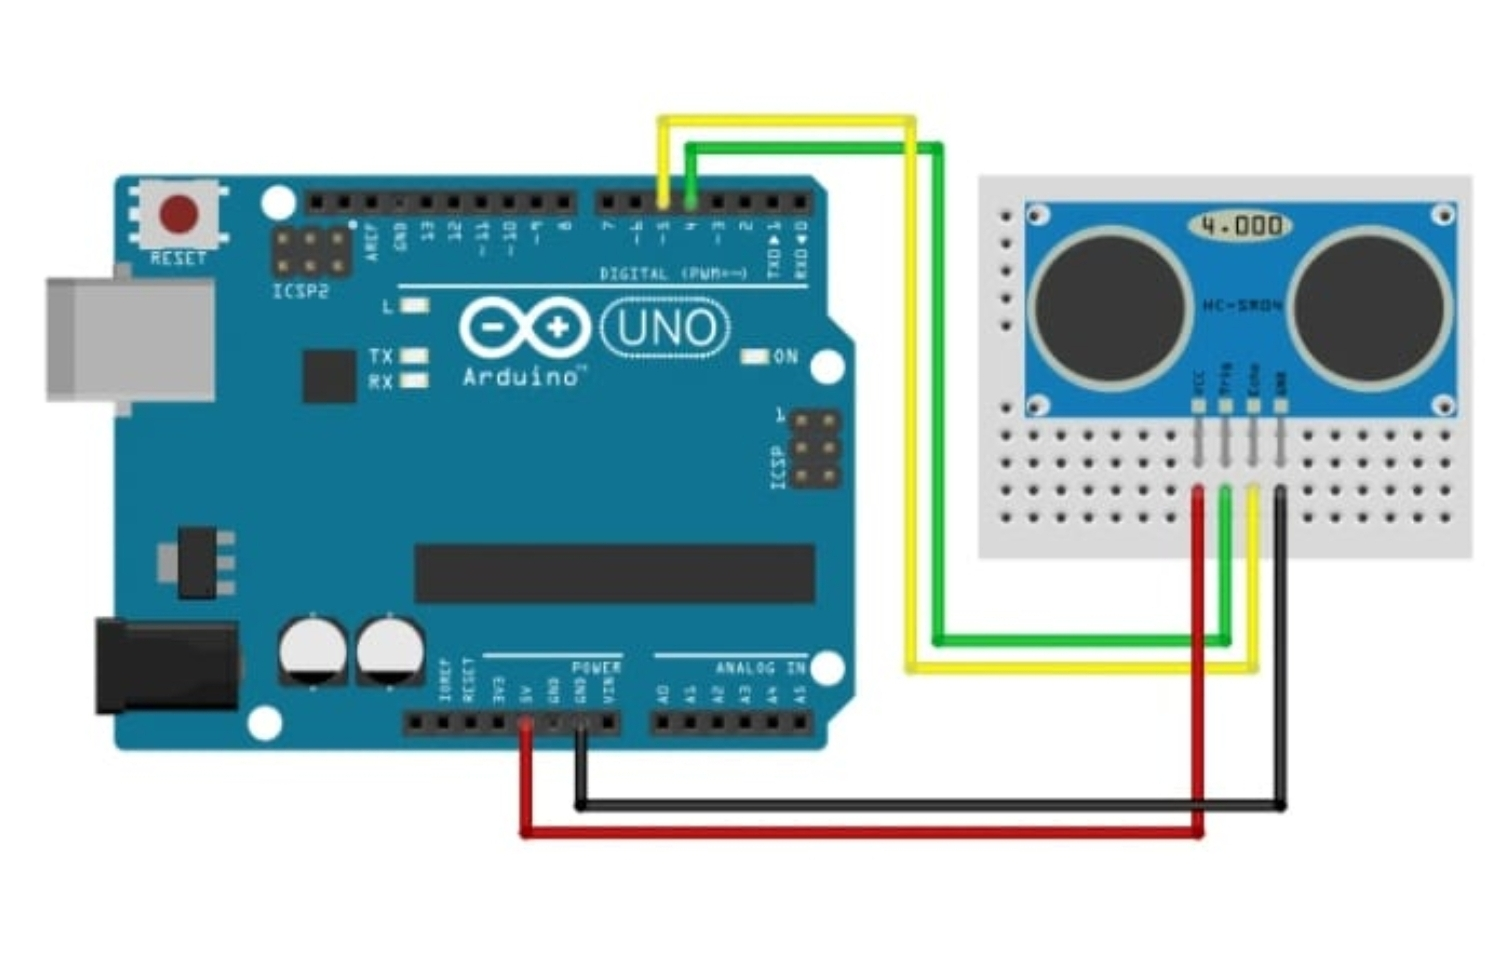
\includegraphics[width=310px]{circuito1.jpg}
  
\end{figure}

    
\end{frame}

\begin{frame}{Arranjo experimental}

    \begin{figure}
  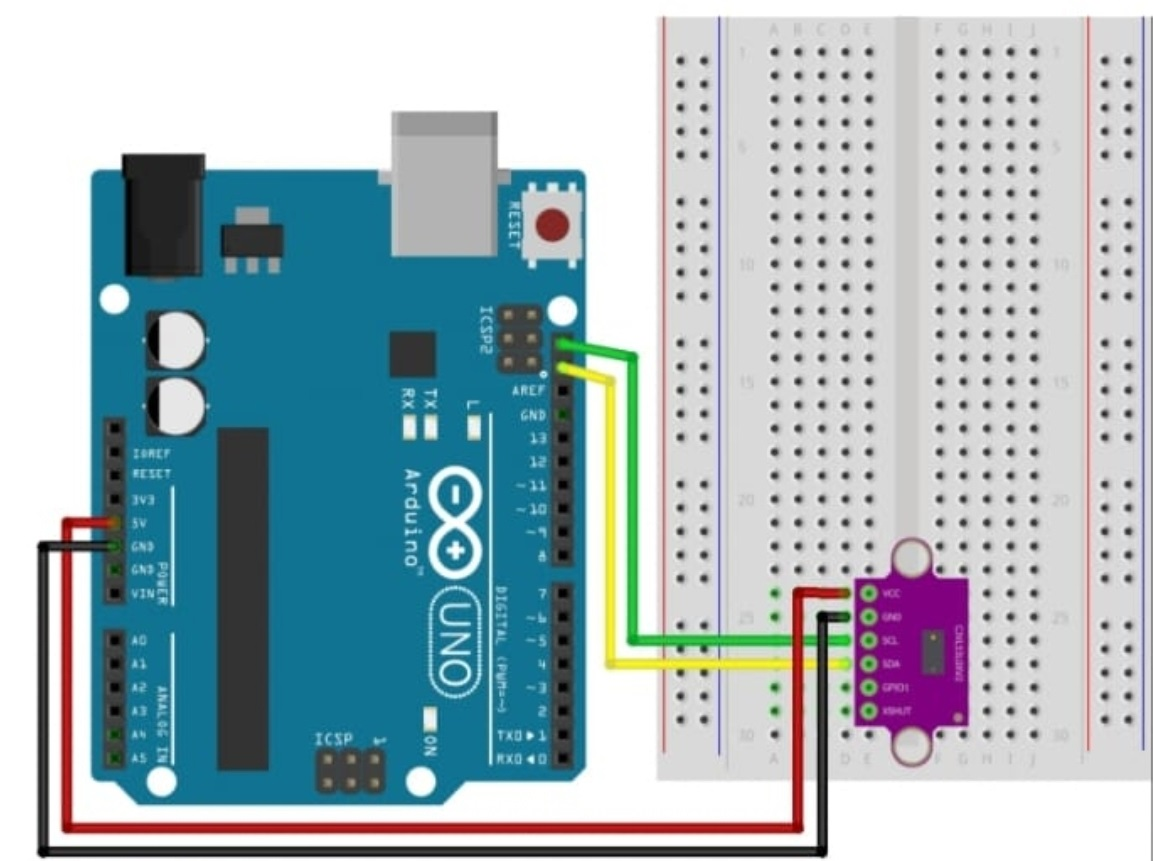
\includegraphics[width=250px]{circuito2.jpg}
  
\end{figure}

    
\end{frame}

\begin{frame}{Arranjo experimental}

    \begin{figure}
  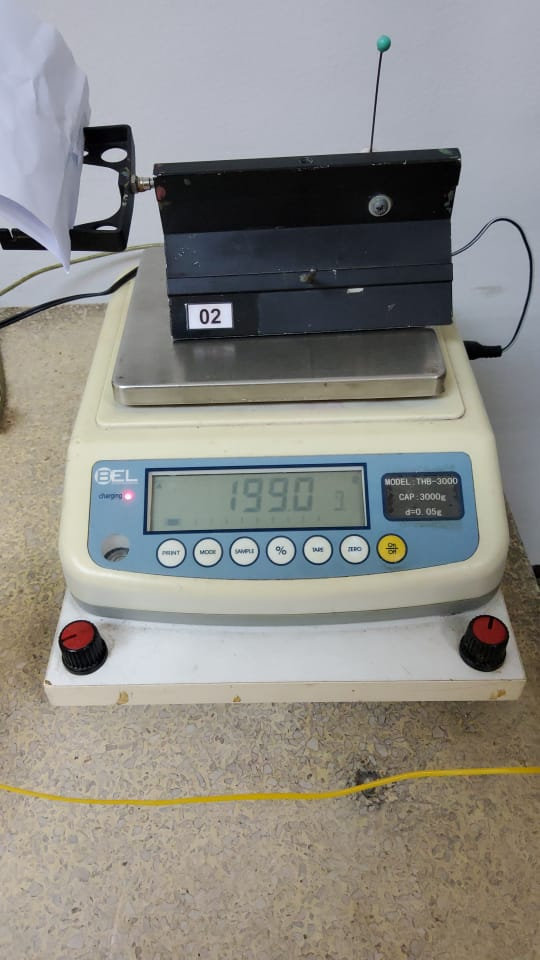
\includegraphics[width=120px]{1a4c4a09-f01b-4def-b72b-968d90990223.jpg}
  
\end{figure}

    
\end{frame}

\begin{frame}{Resultados}
    
     \begin{figure}
  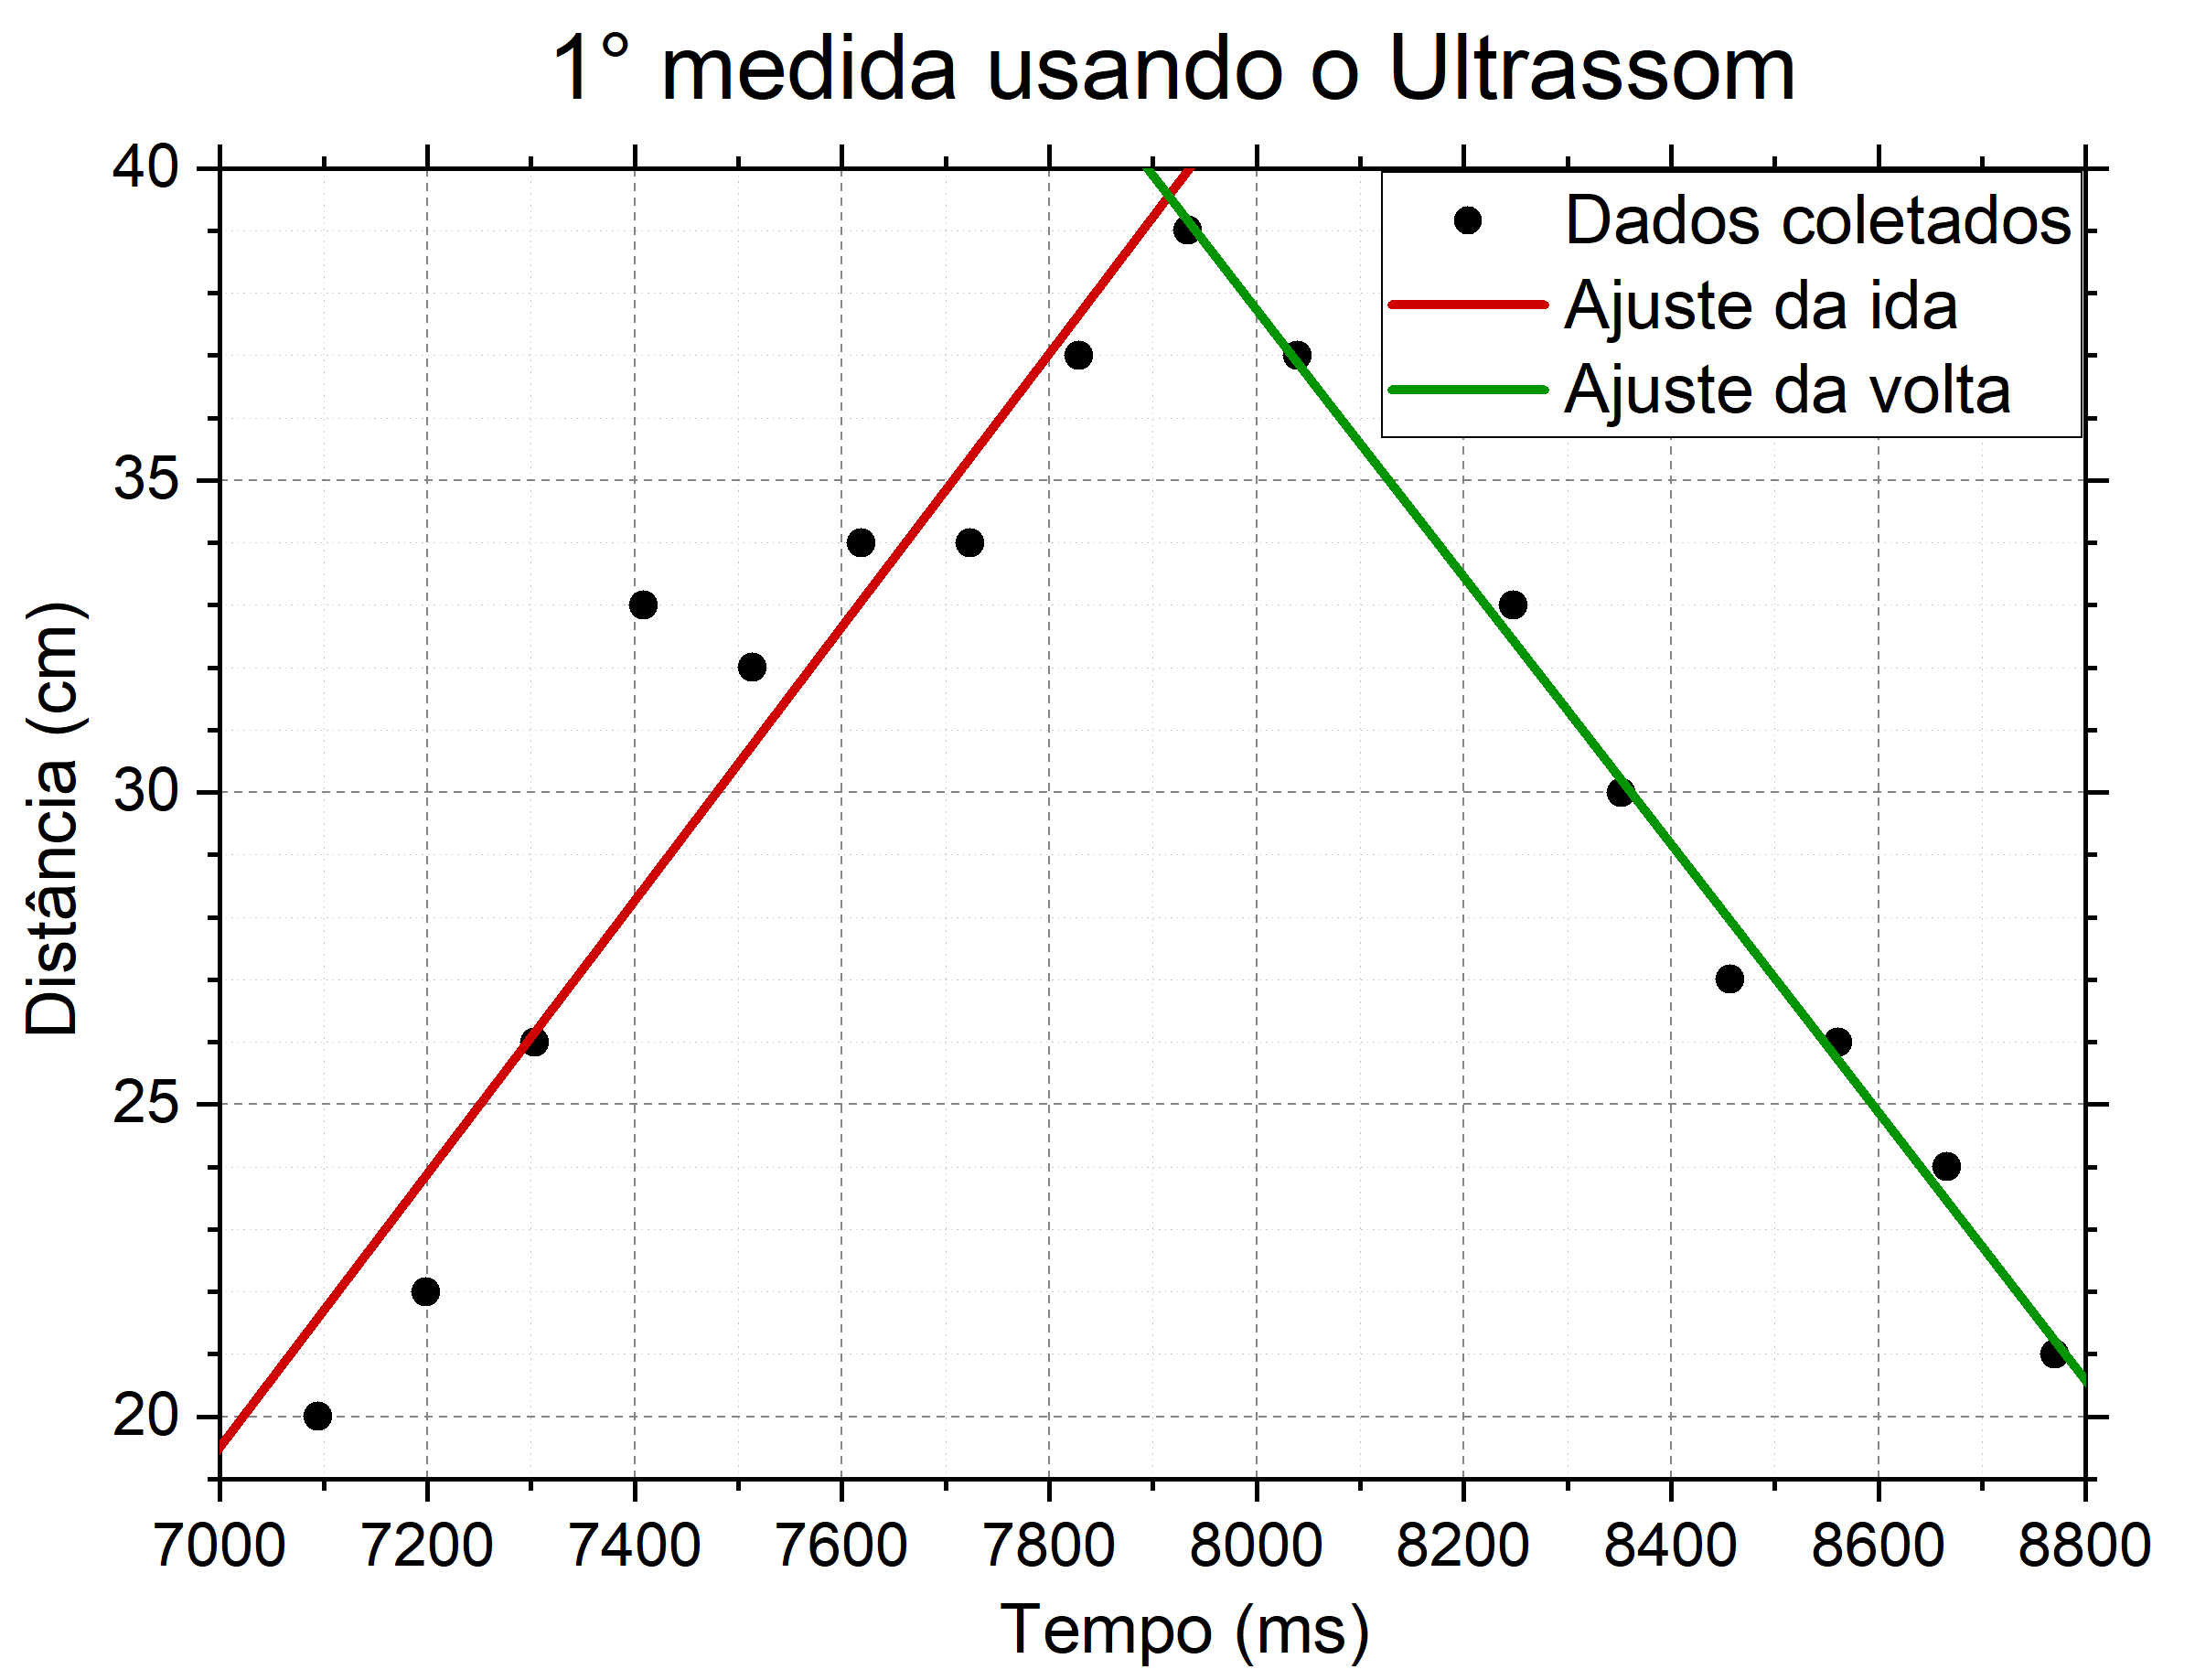
\includegraphics[width=\linewidth]{GraficoUltrassom1.png}
\end{figure}
    
\end{frame}

\begin{frame}{Resultados}
    
     \begin{figure}
  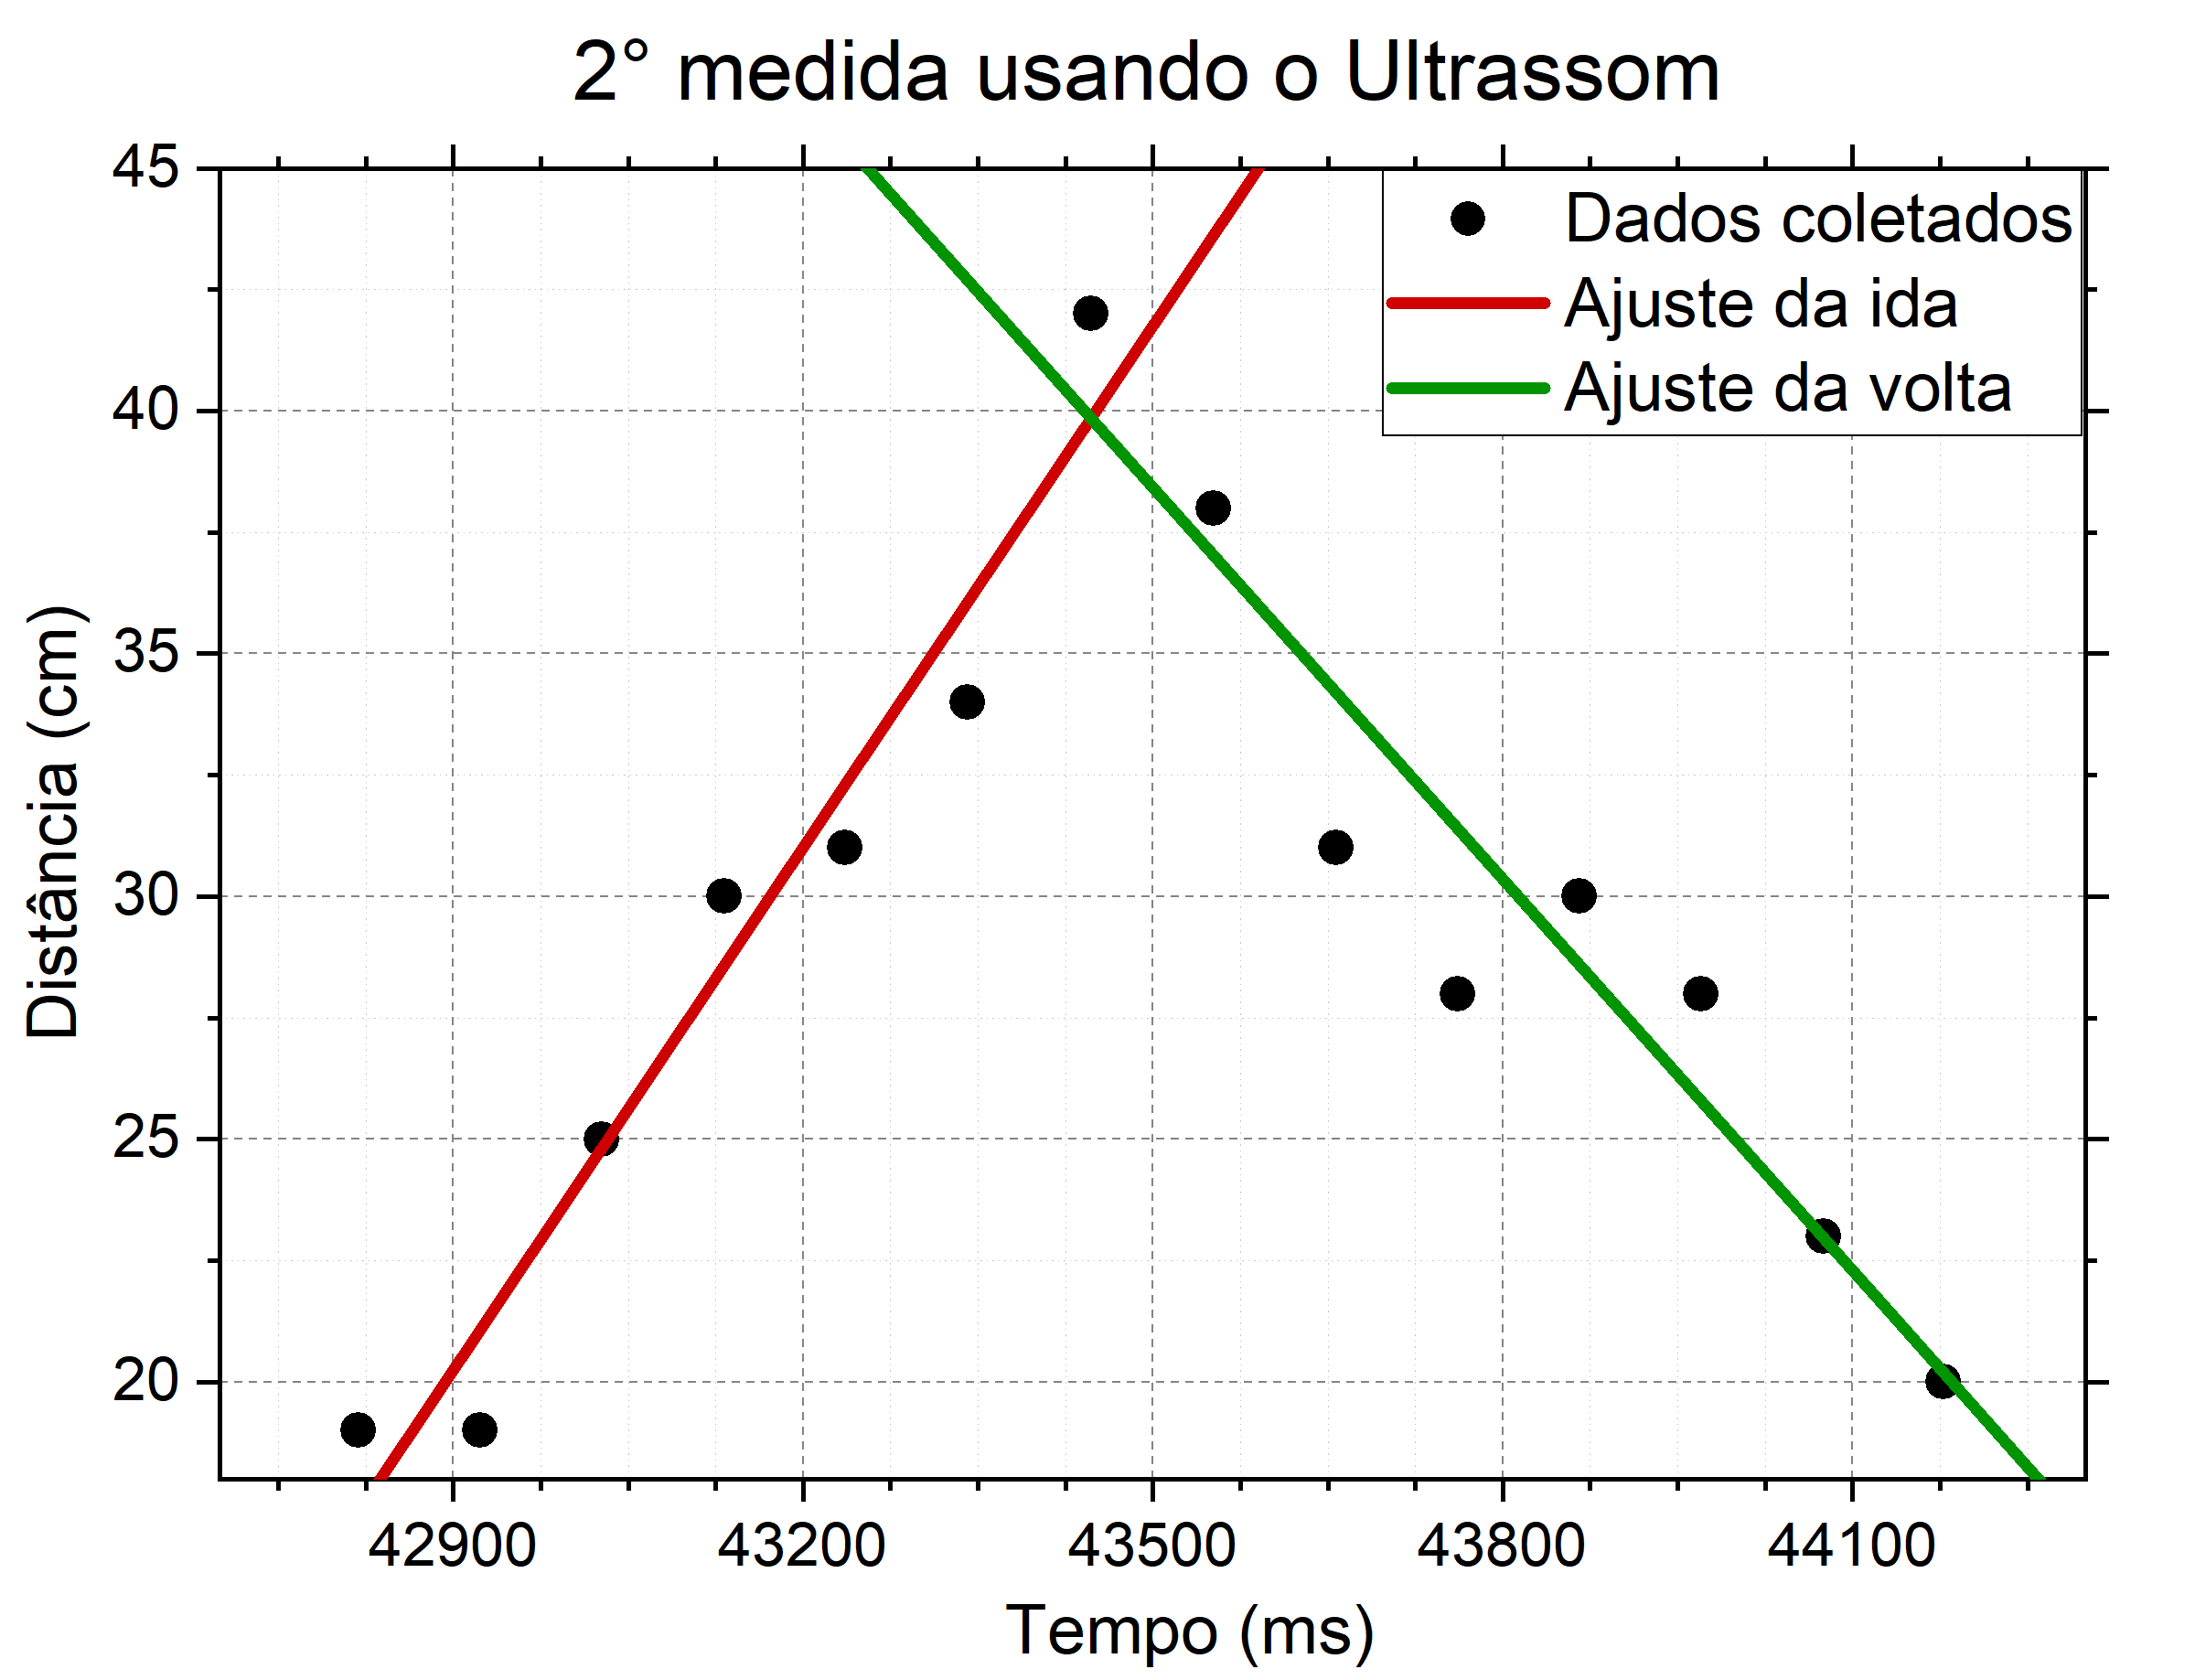
\includegraphics[width=\linewidth]{GraficoUltrassom2.png}
\end{figure}
    
\end{frame}
\begin{frame}{Resultados}
    
     \begin{figure}
  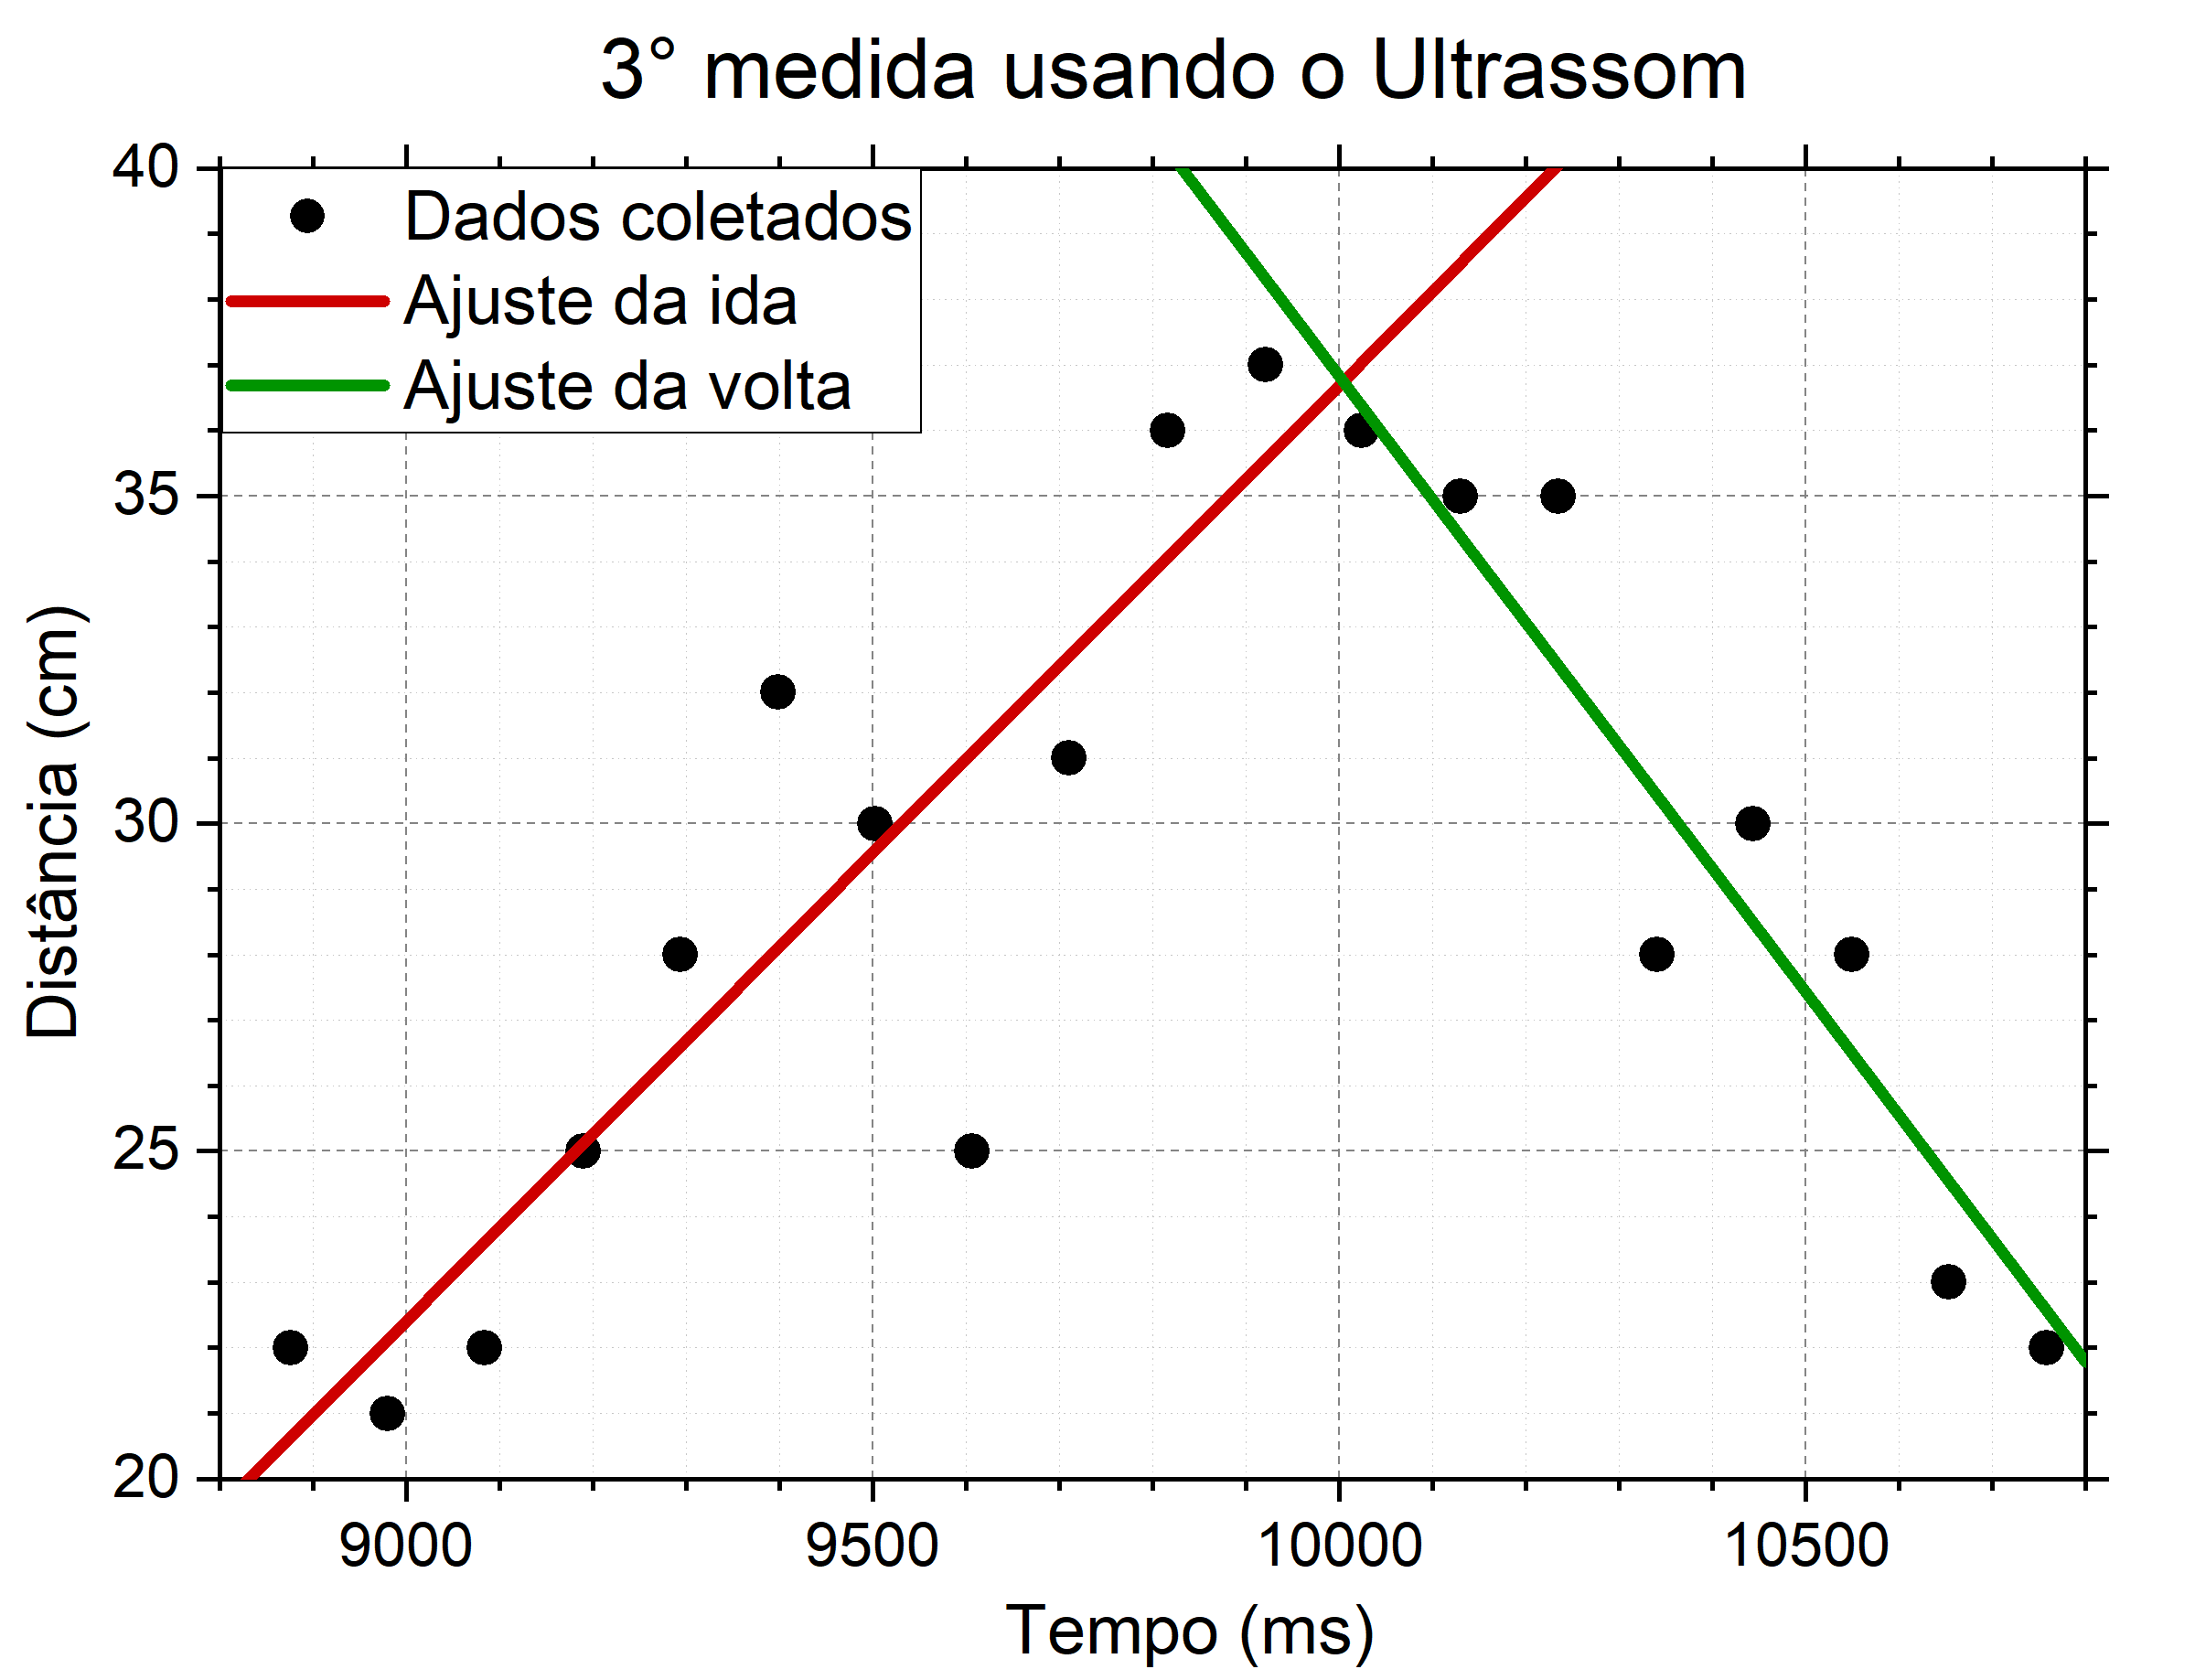
\includegraphics[width=\linewidth]{GraficoUltrassom3.png}
\end{figure}
    
\end{frame}
\begin{frame}{Resultados}
    
     \begin{figure}
  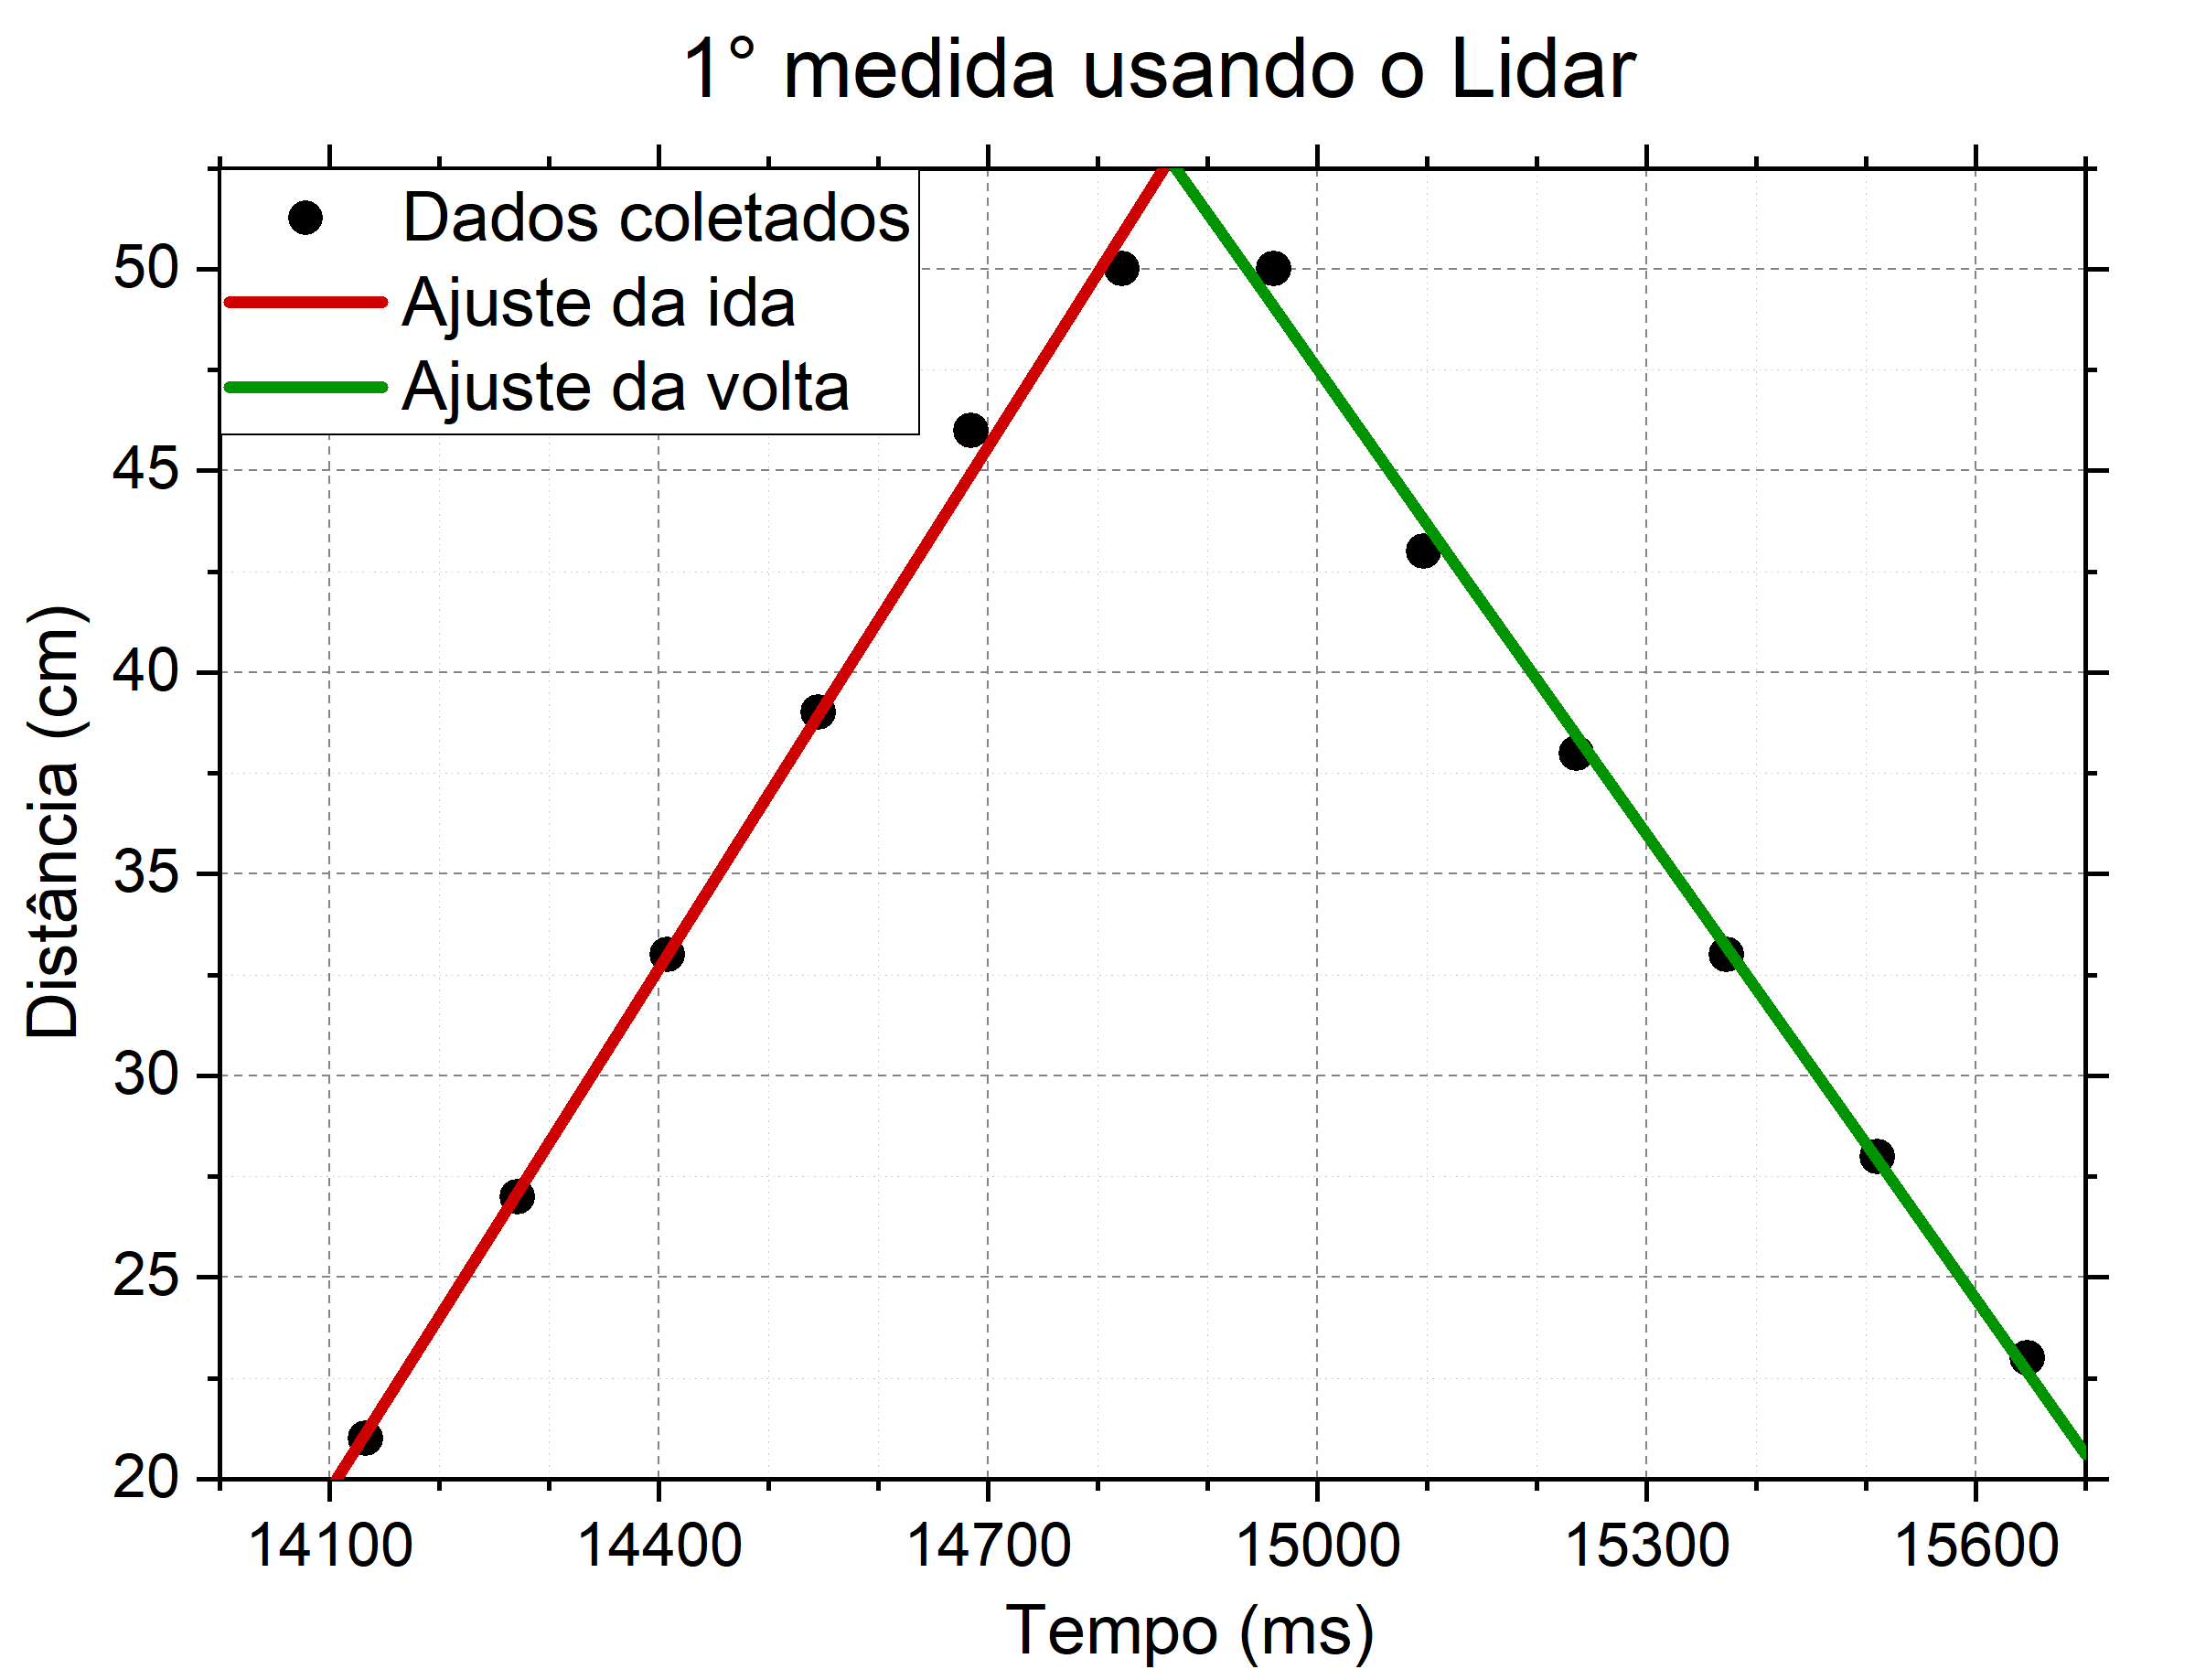
\includegraphics[width=\linewidth]{GraficoLidar1.png}
\end{figure}
    
\end{frame}
\begin{frame}{Resultados}
    
     \begin{figure}
  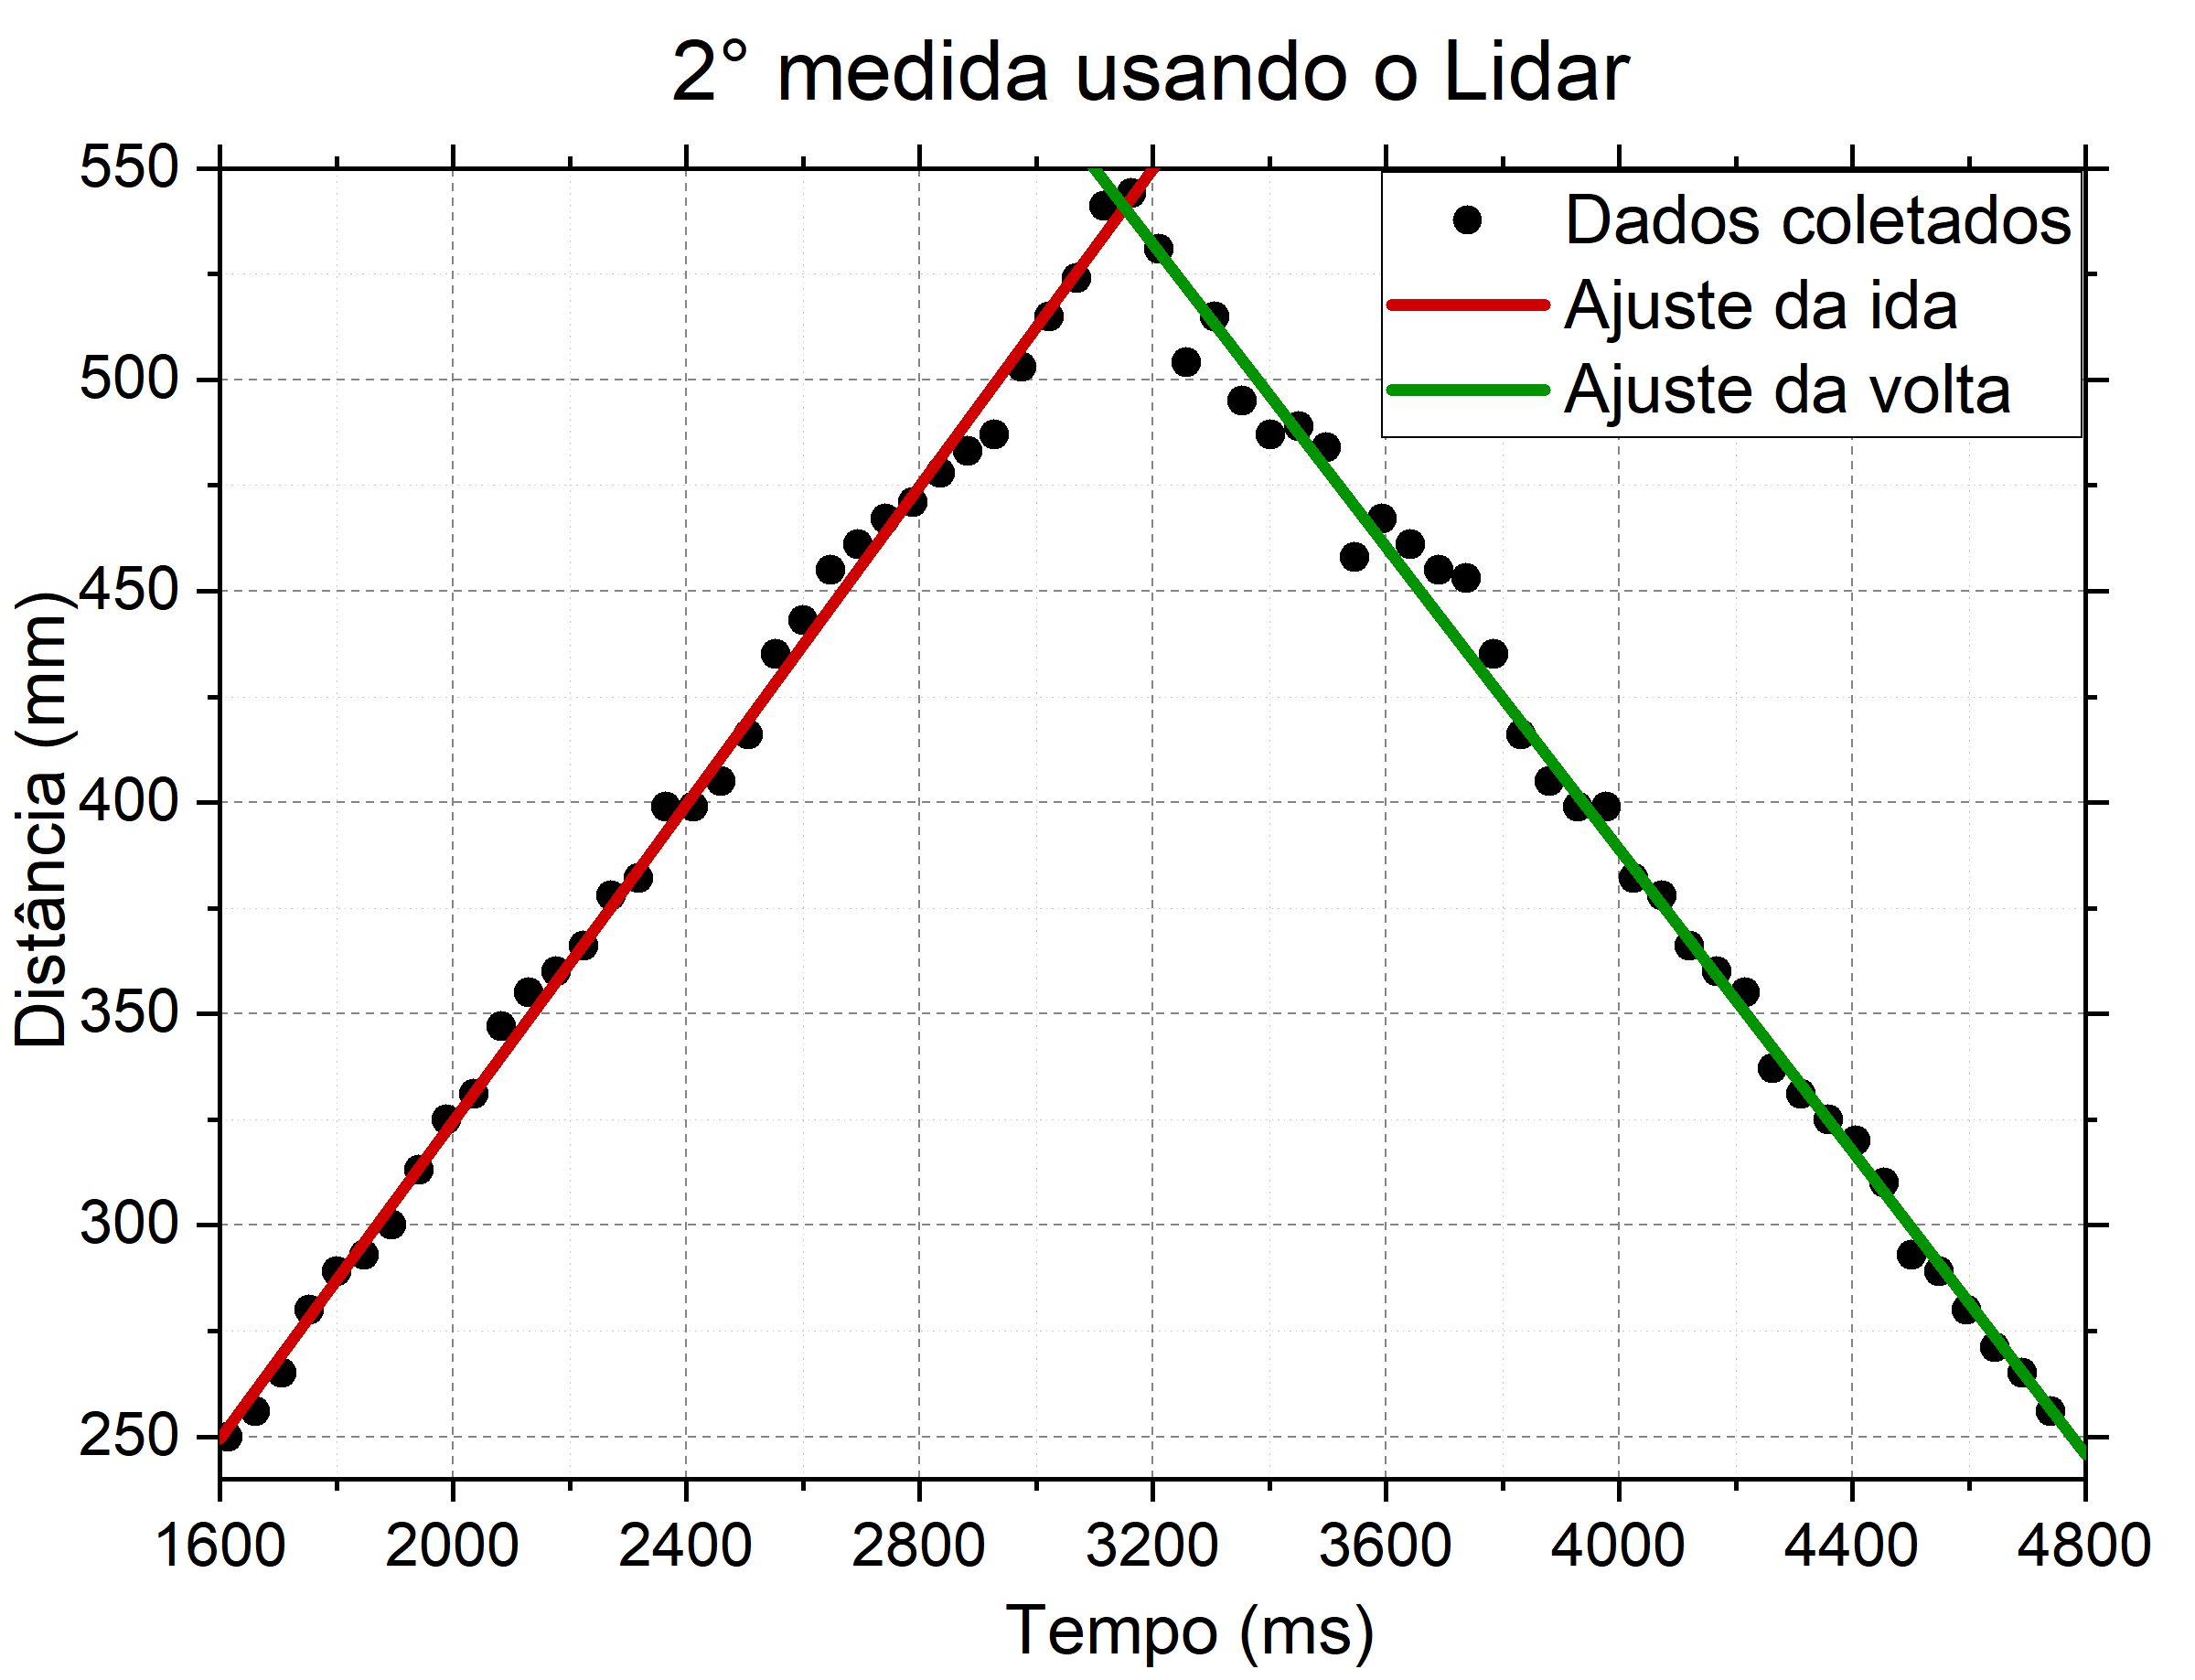
\includegraphics[width=\linewidth]{GraficoLidar2.png}
\end{figure}
    
\end{frame}
\begin{frame}{Resultados}
    
     \begin{figure}
  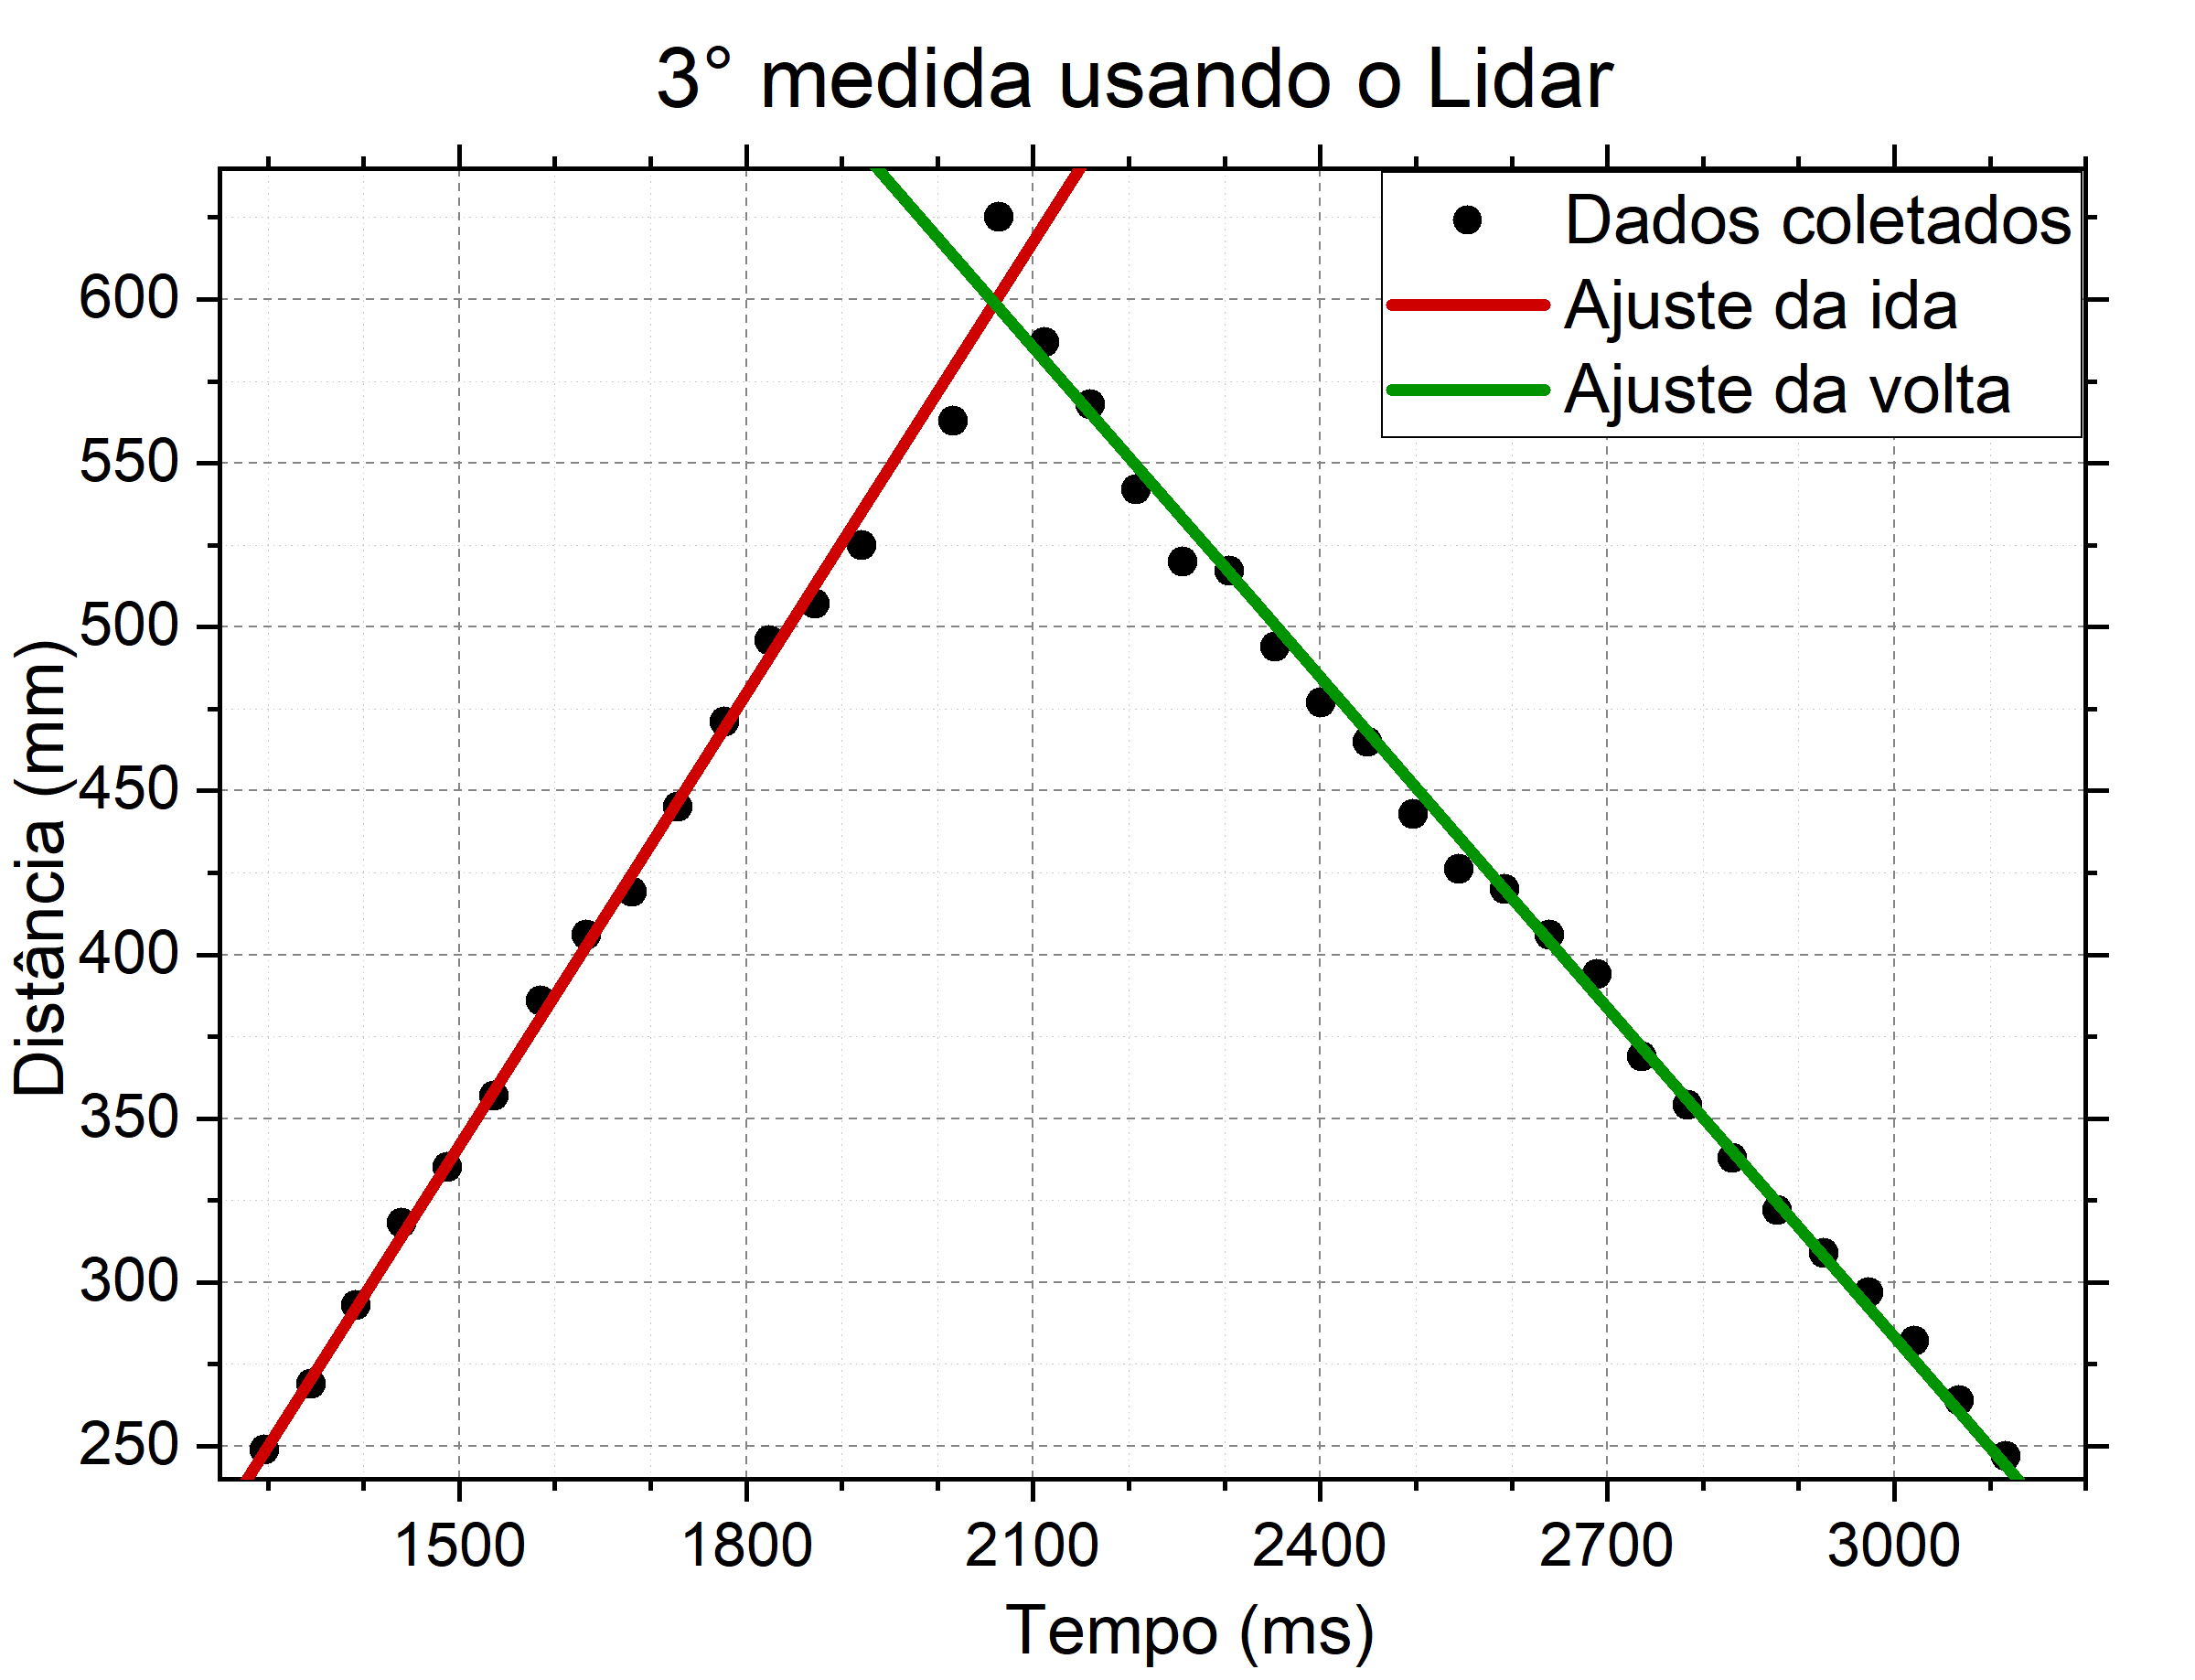
\includegraphics[width=\linewidth]{GraficoLidar3.png}
\end{figure}
    
\end{frame}
\begin{frame}{Resultados}
    
     \begin{figure}
  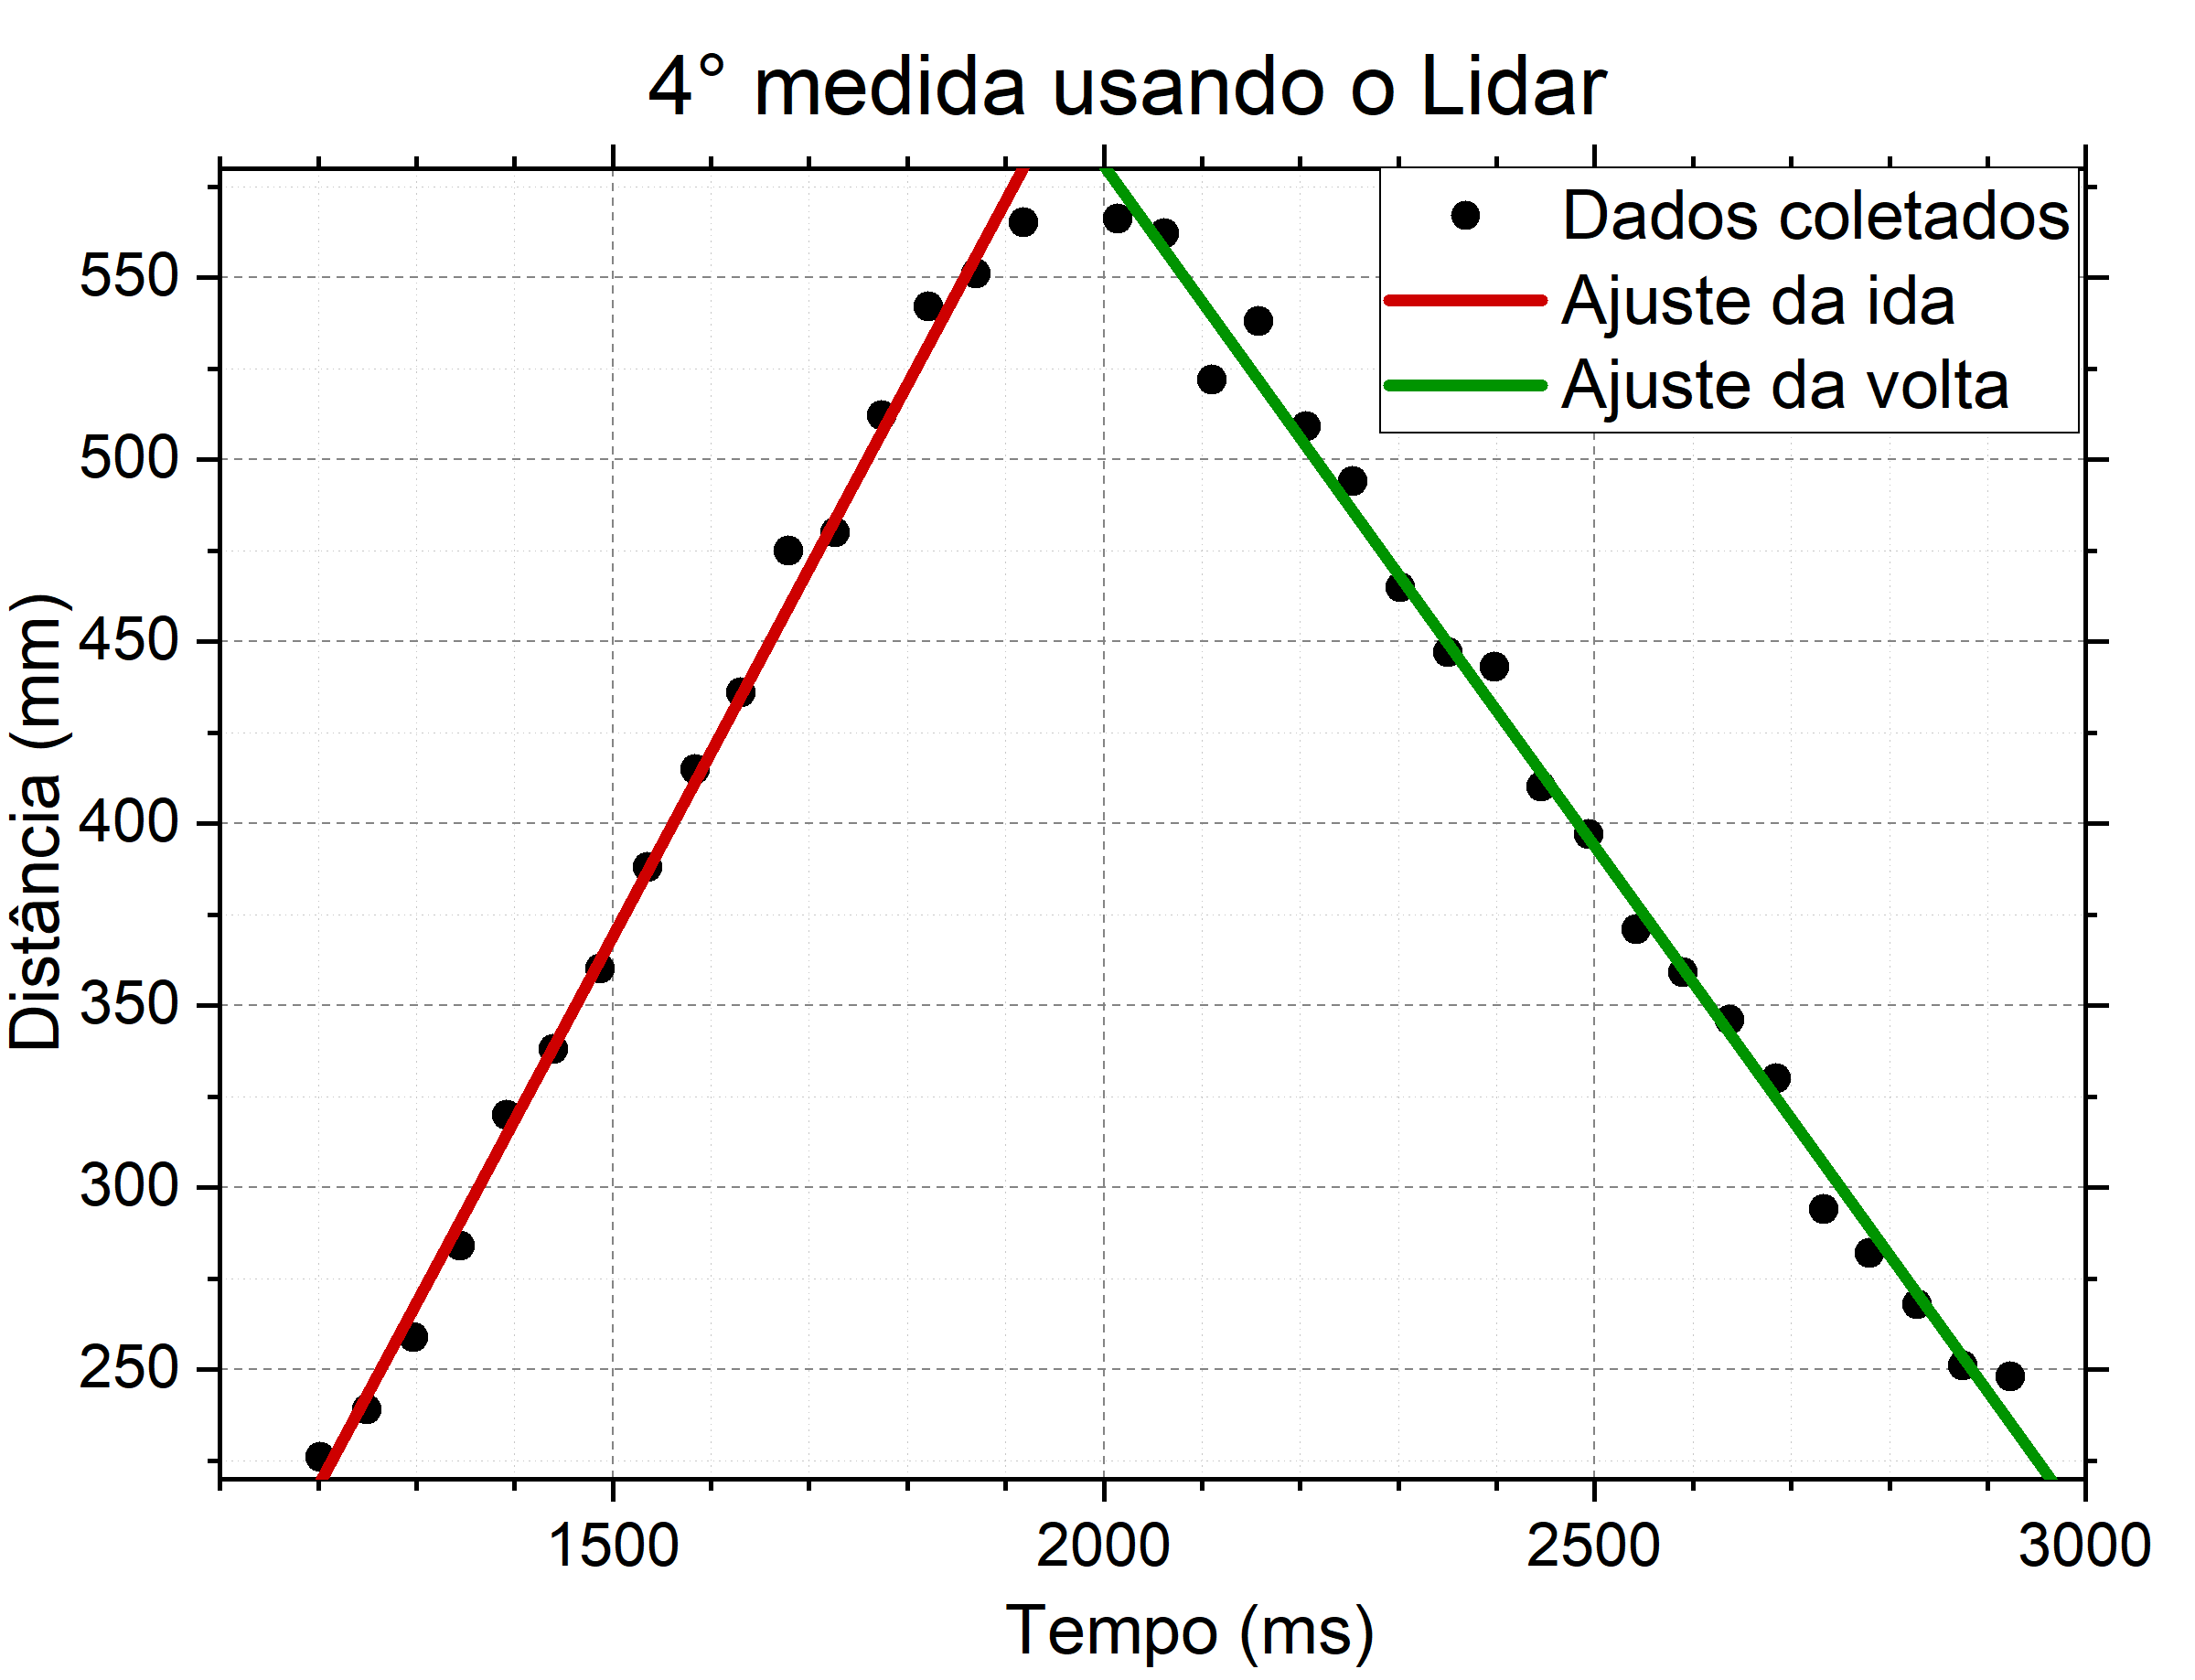
\includegraphics[width=\linewidth]{GraficoLidar4.png}
\end{figure}
    
\end{frame}

\begin{frame}{Resultados}
    
     \begin{figure}
  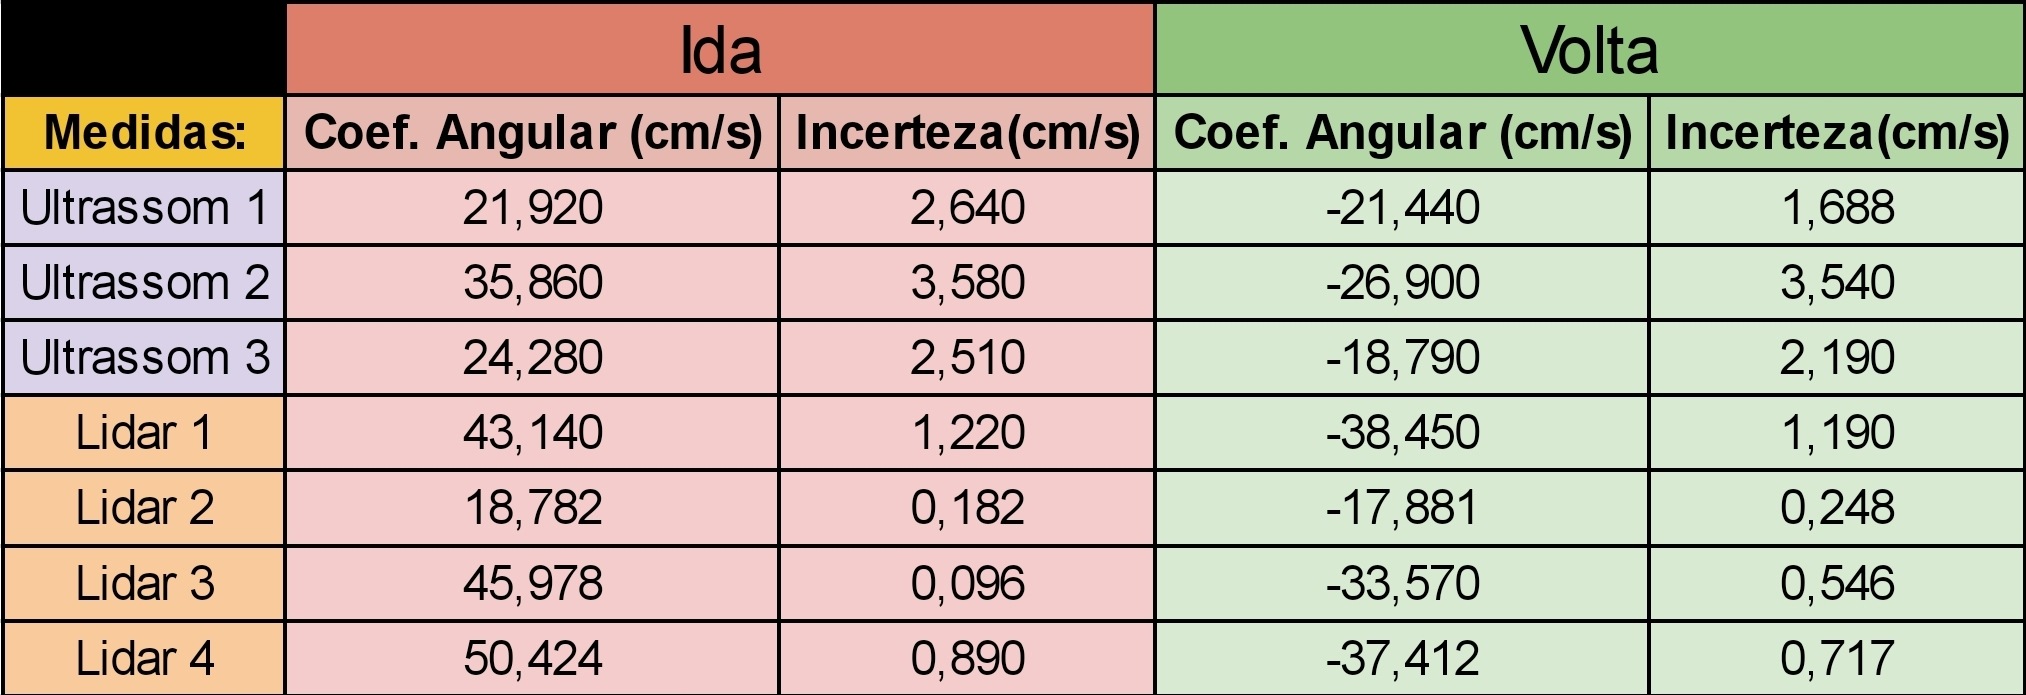
\includegraphics[width=\linewidth]{tabela.jpg}
\end{figure}
    
\end{frame}

\begin{frame}{Análise dos Resultados}

    Considerando um caso ideal em que não há perdas de energia, se espera que:
    $$\dfrac{V_{ida}}{\vert V_{volta}\vert} = 1$$

    Portanto, calculamos isso para cada medida e obtemos a incerteza dessa razão por meio da propagação de incertezas.
    
\end{frame}

\begin{frame}{Análise dos Resultados}
    
     \begin{figure}
  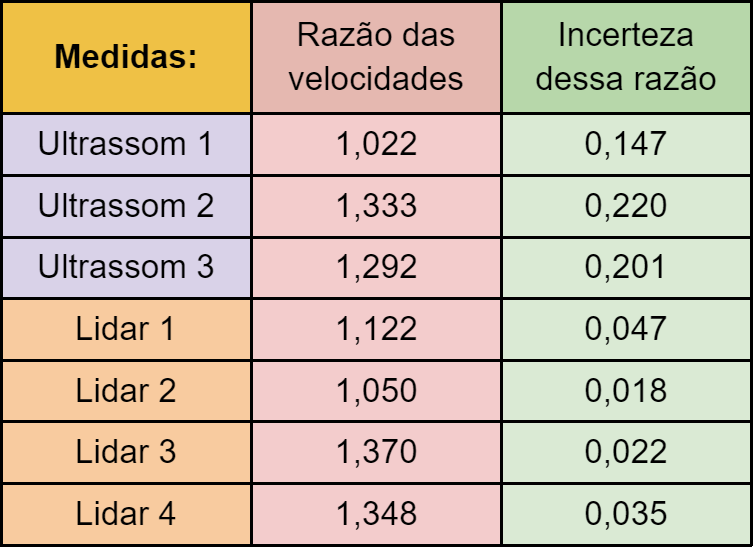
\includegraphics[width=\linewidth]{tabela2.png}
\end{figure}
    
\end{frame}

\begin{frame}{Análise dos Resultados}

    Dessa forma, obtemos que para o sensor de ultrassom:
    $$\dfrac{V_{ida}}{\vert V_{volta}\vert} = 1,165~~\pm~~ 0,104$$
    E para o sensor de infravermelho:
    $$\dfrac{V_{ida}}{\vert V_{volta}\vert} = 1,196~~\pm~~ 0,012$$
    Ambos os valores estão acima do esperado, mas eles fazem sentido, uma vez que há uma certa perda de energia na colisão. Também é possível observar que a incerteza do sensor de infravermelho é $\approx 9$ vezes menor do que a incerteza do ultrassom.
    
\end{frame}

\begin{frame}{Conclusões}

    \begin{itemize}
        \item É possível utilizar os sensores para realizar esse tipo de experimento. 
        \item Os dados obtidos pelo sensor de ultrassom são menos precisos que os dados obtidos pelo sensor de infravermelho.
        \item Sensor de ultrassom não é tão preciso para grandes distâncias.
        \item Com mais ajustes, é um experimento que pode ser replicado em aulas de física experimental. 
    \end{itemize}
    
\end{frame}

\end{document}